\documentclass[10pt,nocopyrightspace]{sigplanconf}


%\usepackage{makeidx}

%\usepackage{amsmath}
%\usepackage{amssymb}

%\usepackage{multicol}
\usepackage{multirow}
%\usepackage{graphicx}
\usepackage{epsfig}

\usepackage{color}
\usepackage{subfigure}
%\usepackage{fancybox}
\usepackage{fancyvrb}

%\usepackage{rotating}

\usepackage{fancyhdr}


\DefineVerbatimEnvironment{colorcode}%
        {Verbatim}{fontsize=\small,commandchars=\\\{\}}   

\definecolor{DikuRed}{RGB}{130,50,32}
\newcommand{\emp}[1]{\textcolor{DikuRed}{ #1}}
\definecolor{CosGreen}{RGB}{10,100,70}
\newcommand{\emphh}[1]{\textcolor{CosGreen}{ #1}}


\newcommand{\mymath}[1]{$ #1 $}
\newcommand{\myindx}[1]{_{#1}}
\newcommand{\myindu}[1]{^{#1}}
\newcommand{\mymathbb}[1]{\mathbb{#1}}

\newcommand{\Figures}[1]{../Figures/}

\hyphenation{in-de-pen-dence}
\hyphenation{pa-ra-lle-lize}
\hyphenation{sub-scrip-ted}
\hyphenation{sub-scrip-ted}
\pagestyle{plain}

\begin{document}

\thispagestyle{fancy}

\def\ieeenotice{978-1-4799-8161-8/15/\$31.00 {\copyright}2015 IEEE}
\def\confinfo{2015 IEEE/ACM International Symposium on Code Generation and Optimization}
\lfoot{\confinfo\\\ieeenotice} \cfoot{}
\renewcommand{\headrulewidth}{0pt} 


\special{papersize=8.5in,11in}
\setlength{\pdfpageheight}{\paperheight}
\setlength{\pdfpagewidth}{\paperwidth}
 

\title{Scalable Conditional Induction Variables (CIV) Analysis}   

\authorinfo{Cosmin E. Oancea}
           {Department of Computer Science\\University of Copenhagen}
           {cosmin.oancea@diku.dk}
\authorinfo{Lawrence Rauchwerger}
           {Department of Computer Science and Engineering\\Texas A \& M University}
           {rwerger@cse.tamu.edu}


\maketitle

\begin{abstract}

Subscripts using induction variables that cannot be expressed 
as a formula in terms of the enclosing-loop indices appear in 
the low-level implementation of common programming abstractions 
such as filter, or stack operations and pose significant challenges 
to automatic parallelization. Because the complexity of such induction 
variables is often due to their conditional evaluation across the 
iteration space of loops we name them 
{\em Conditional Induction Variables} ({\sc civ}).

This paper presents a flow-sensitive technique that summarizes 
both such {\sc civ}-based and affine subscripts to program level,
using the same representation. Our technique requires no 
modifications of our dependence tests, which is agnostic to the 
original shape of the subscripts, and is more powerful %a technique
than previously reported dependence tests that rely on the pairwise
disambiguation of read-write references.

We have implemented the {\sc civ}  analysis in our parallelizing compiler and
evaluated its impact on five Fortran benchmarks. We have found that
that there are many important loops using {\sc civ} subscripts and that
our analysis can lead to their scalable parallelization. This in turn has led
to the parallelization of the benchmark programs they appear in. 
\end{abstract}


%\category{D.1.3}{Concurrent Programming}{Parallel Programming}
%\category{D.3.4}{Processors}{Compiler}
%\terms{Performance, Design, Algorithms}
%\keywords{array-reference summaries, conditional induction variables}


\section{Introduction}

An important step in the automatic parallelization  of loops
is the analysis of induction variables and their transformation into a
form that allows their parallel evaluation. In the case of ``well behaved''
induction variables, that take monotonic values with a constant stride,
their generating sequential recurrence can be 
substituted with the evaluation of closed form expression of the loop indices.
This transformation
enables the parallel evaluation of the induction variables. When these variables
are used to form addresses of shared data structures, the memory references
can be statically analyzed and possibly parallelized. Thus we can conclude 
that the analysis of induction-variables use is crucial %and parallelization 
to loop  dependence
analysis~\cite{BanerjeeIneqTest,FeautrierDataflow,Pugh92theomega} 
and their subsequent parallelization. 


% 

\begin{figure}
\begin{minipage}{0.6\columnwidth}
\begin{colorcode}
k = k0    \emphh{\em Ind.} k = k0        
DO i =1,N \emphh{\em Var.} DO i = 1, N      
  k = k+2   \emphh{\mymath{\Rightarrow}}   a(k0+2*i)=.. 
  a(k)=.. \emphh{\em Sub.} ENDDO         
ENDDO           k=k0+MAX(2N,0)
   (a)              (b) 
\end{colorcode}
\end{minipage}
\begin{minipage}{0.35\columnwidth}
\begin{colorcode}
DO i = 1, N
 IF(cond(b(i)))THEN 
    civ = civ+1 \emp{\mymath{\Rightarrow}{\em?}} 
    a(civ) = ...
ENDIF ENDDO
      (c)
\end{colorcode}
\end{minipage}
\caption{Loops with affine and {\sc civ} array accesses.}
\label{fig:introEg}
\vspace{-2ex}
\end{figure}


For example, the loop in Figure~\ref{fig:introEg}(a) increments
by two the value of {\tt k} (produced by the previous iteration),
and updates the {\tt k$^{th}$} element of array {\tt a}. 
%
The uniform incrementation of {\tt k} allows to substitute this
recurrence on {\tt k} with its closed-form equivalent {\tt k0+2*i},
which enables its independent evaluation by all iterations.
More importantly, the resulted code, shown in Figure~\ref{fig:introEg}(b),
allows the compiler to verify that the set of points written by any
distinct iterations {\em do not overlap}, a.k.a., output independence: 
{\tt k0+2*i$_1$~=~k0+2*i$_2$ $\Rightarrow$ i$_1$=i$_2$}. 
It follows that the loop in Figure~\ref{fig:introEg}(b) can be safely
parallelized. 


A known difficulty in performing this analysis arises when
subscripts use scalars that do not form a uniform recurrence,
i.e., their stride (increment) is not constant across iteration space of 
the analyzed loop. 
We name  such variables 
{\em conditional induction variables} or {\sc civ} 
because they are typically updated  (only) on some of 
the possible control-flow paths of an iteration.
%
For example, the loops in Figures~\ref{fig:introEg}(a)~and~(c) are 
similar, except that in (c) both {\tt civ} and the array update are 
performed only when condition {\tt cond(b(i))} holds.  
Although the recurrence computing {\tt civ} values can still 
be parallelized via a scan~\cite{segScan} (prefix sum) precomputation, 
neither {\sc civ} nor the subscript can be summarized as affine 
expressions of loop index {\tt i}, and hence the previous technique 
would fail.  
 
{\em This paper} presents a novel induction-variable analysis that allows
both affine and {\sc civ} based subscripts to be summarized at program level,
using {\em one common representation}.

%PaduaStackArr, % Blume95symbolicrange 
Current solutions~\cite{Blume94RangeTest,SeqVars,VEG,PaduaDemDrInterproc,CohenBeyondMon}
use a two-step approach:
First, {\sc civ} scalars are recognized and their properties, such as 
monotonicity and the way they evolve inside and across iterations, are inferred.   
Intuitively, in our example, this corresponds to determining that 
the values of {\tt civ} are increasing within the loop with step 
at most $1$.
This paper does not contribute to this stage, but  
exploits previously developed techniques~\cite{VEG}.
%
Second and more relevant, each pair of read-write subscripts is
disambiguated, by means of {\em specialized} dependency tests that exploit the
{\sc civ}'s properties. 
In our example, the cross-iteration monotonicity of the {\sc civ} values 
dictates that the {\sc civ} value, named {\tt civ$_2$} after being incremented 
in some iteration {\tt i$_2$} is strictly greater than the value,
named {\tt civ$_1$} of any previous iteration {\tt i$_1$}.
It follows by induction that the update of {\tt a(civ)}
cannot result in cross-iteration (output) dependencies, i.e.,
the system {\tt civ$_2$-civ$_1 \geq 1$} and {\tt civ$_2 = $civ$_1$}
has no solution. 

Other summarization techniques~\cite{SUIF,LMAD,CosPLDI} aggregate 
array references across control-flow constructs, e.g., branches, loops, and  
model dependency testing as an equation on the resulted abstract sets.
In practice, they were found to scale better than previously developed
analysis based on pairwise accesses~\cite{SUIF}, 
but they do not support {\sc civ}s.

This paper proposes an extension to summary-based analysis 
that allows  {\sc civ} based subscripts to use the same representation  
as the affine subscripts. This enables scalable memory reference analysis
without modification of the previously developed dependency tests.
%
The gist of our technique is to aggregate symbolically the {\sc civ} 
references on every control-flow path of the analyzed loop, in terms
of the {\sc civ} values at the entry and end of each iteration or loop.
The analysis succeeds if (i) the symbolic-summary results are identical 
on all paths and (ii) they can be aggregated across iterations 
in the interval domain. 

We demonstrate the technique on the loop in Figure~\ref{fig:introEg}(c),
where we use {\tt civ$_\mu^i$} and {\tt civ$_b^i$} to denote the values of 
{\tt civ} at the entry and end of iteration {\tt i}, respectively.
%
On the {\tt THEN} path, i.e., {\tt cond(b(i))} holds, the write set 
of array {\tt a} is interval $W_i=${\tt [civ$_\mu^i$+1,civ$_b^i$]}, 
i.e., point {\tt \{civ$_\mu^i$+1\}}, because the incremented value 
of {\tt civ} is live at the iteration end. 
%
On the {\tt ELSE} path, the write set of {\tt a} is the empty set.
For uniformity of representation we express this empty set as an interval
with its lower bound
greater than its upper bound. In particular, the interval of the
{\tt THEN} path matches, because {\tt civ} is not updated and so
{\tt civ$_\mu^i$+1>civ$_b^i$}.


Aggregating $W_k$ across the first {\tt i-1} iterations results in
$\cup_{k=1}^{i-1}W_k \ = \ $ {\tt [civ$_\mu^1$+1,civ$_\mu^i$]}, 
where we have used {\tt civ} values'
monotonicity and the implicit invariant {\tt civ$_b^{k-1}\equiv$civ$_\mu^{k}$},
i.e., the {\tt civ} value at an iteration end is equal to the {\tt civ}
value at the entry of the next iteration. 
%
%Since in many cases it is not possible to derive an accurate result,
%our analysis computes a pair of under/overestimate summaries, which
%are enough in practice to verify the needed invariants.
%
As a last step, program invariants are modeled as abstract-set equations
that do not depend on the original-subscript shape, i.e., 
{\sc civ}-based or affine. 
%
In our example, the output independence equation:\\
$(\cup_{k=1}^{i-1}W_k)\cap W_i${\tt=[civ$_\mu^1$+1,civ$_\mu^i$]}$\cap$
{\tt [civ$_\mu^i$+1,civ$_b^i$]=}$\emptyset,\forall\mbox{\tt{}i}$,
verifies that the write set of any iteration {\tt i} does not overlap
the write set of all previous iterations, and, by induction,
that no distinct iterations write a common element of {\tt a}.


Our technique is well integrated 
into the \textsc{Parasol} branch of the Polaris~\cite{Blume94automaticdetection} 
{\tt Fortran} compiler. We  use {\em hybrid analysis} to
verify dataset-sensitive invariants % (statically-unverifiable)  
at runtime by evaluating a sequence of sufficient-conditions 
 of increasing complexity.
These conditions (predicates) are statically synthesized from the summary 
equations that model the relevant invariants 
%
Our existing hybrid analysis did not require modifications
but has benefited from our technique: 
%
First, our analysis simplifies {\sc civ}-summary expressions
enabling successful verification of the relevant invariants.
Second, our analysis extracts the slice of the loop that computes
the {\sc civ} values and evaluates it in parallel before loop
execution. This allows: 
  (i) runtime verification of {\sc civ} monotonicity whenever 
          this cannot be statically established,  
 (ii) sufficient conditions for safe parallelization to 
          be expressed in terms of the {\sc civ} values at loop's 
          entry, end, and anywhere in between, and 
(iii) safe parallelization in the simple case when
        {\sc civ} are not used for indexing.
The latter is not reported in related work.
%
%{\sc civ} summaries have a wider applicability than 
%dependency testing, e.g., in the context of array {\sc ssa}.
%
In summary, main contributions are:
\begin{itemize}
    \item A flow-sensitive analysis that extends 
            program level summarization to support {\sc civ}-based 
            indices and leads to the parallelization of
            previously unreported loops, 

    \item A non-trivial code generation that separates the 
            program slice that performs the parallel-prefix-sum
            evaluation of the {\sc civ} values 
            from the main (parallel) computation in which 
            they are inserted.
            %% Previous solutions do not support this, 
            %% albeit it is necessary at least when {\sc civ}s are 
            %% not used for indexing.
            
    \item An evaluation of five difficult to parallelize benchmarks 
            with important {\sc civ}-subscripted loops, which measures 
            all runtime overheads and shows application level speed-ups 
            as high as $7.1\times$ and on average $4.33\times$ on $8$ cores.
%            This includes all runtime overheads, 
%            e.g., {\sc civ}-values computation, which are either 
%            negligible or scale well with the degree of parallelism.
%
\end  {itemize}

Speedups of two of this paper benchmarks shown were also reported 
in~\cite{CosPLDI}. They were obtained in part by using the {\sc civ} 
technique that is {\em presented here for the first time}.


\section{An Intuitive Demonstration}
\label{Intro:RelAppLim}

Figure~\ref{fig:codeActforCorrec}(a) shows a simplified version of
loop {\tt CORREC\_do401} from {\sc bdna} benchmark, 
as an example of non-trivial loop that uses both {\sc civ} and affine-based
subscripts.   Variable {\tt civ}  uses (gated) 
single-static-assignment ({\sc ssa}) notation~\cite{GatedSSA}: 
%
For example, statement {\tt civ@2=$\gamma$(i.EQ.M,civ@1,civ@4)}
has the semantics that variable {\tt civ@2} takes, depending 
on the evaluation of {\tt i.EQ.M}, either the value of {\tt civ@1} for 
the first iteration of the loop that starts at {\tt M}, or the value of 
{\tt civ@4} for all other iterations. For simplicity we omit the gates 
in the figure and use only read and write reference sets
(but our implementation uses read-only, write-first, read-write sets).

\begin{figure}
\begin{minipage}{0.49\columnwidth}
\begin{colorcode}
civ@1 = Q
DO i = M, N, 1
 civ@2=\mymath{\gamma}(civ@1,civ@4)
 .. = {\bf X}(i) ..
 IF C(i) .GT. 0 THEN
  DO j = 1, C(i), 1
   IF(..){\bf{}X}(j+civ@2       )=..
   IF(..){\bf{}X}(j+civ@2+  C(i))=..
   IF(..){\bf{}X}(j+civ@2+2*C(i))=..
  ENDDO
  civ@3 = 3*C(i) + civ@2
 ENDIF
 civ@4=\mymath{\gamma}(civ@3,civ@2)
ENDDO
civ@5=\mymath{\gamma}(civ@4,civ@1)
  
            (a)
\end{colorcode}
\hspace{2ex}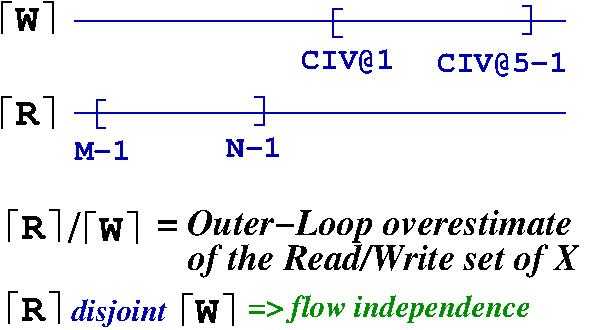
\includegraphics[width=1\textwidth]{\Figures/CorrecRWsets.jpg}
\end{minipage}
\begin{minipage}{0.45\columnwidth}
\begin{colorcode}
      VEG annotated with 
      CIV-based summaries 
      at Gated-SSA Path, 
         Iteration and 
         Loop Levels
\end{colorcode}
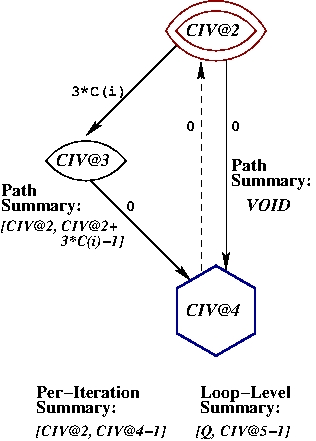
\includegraphics[width=1.15\textwidth]{\Figures/VEG_CORREC.jpg}
\begin{colorcode}
                (b)
\end{colorcode}
\end{minipage}
\caption{(a) Loop {\tt CORREC\_do401} and (b) its Value Evolution Graph ({\sc veg}),
                (from {\sc bdna}, {\sc Perfect-Club}).}
\label{fig:codeActforCorrec}
\end{figure}

Parallelizing loop {\tt CORREC\_do401} in Figure~\ref{fig:codeActforCorrec}(a)
requires verifying two invariants: The first refers to disproving 
cross-iteration true and anti dependencies. For such dependencies to occur it 
is necessary that there exists a memory location that is both read and written,
and we plan to disprove this by verifying that the overestimates of the read 
and write sets (of subscripts) of {\tt X}, aggregated at the outer-loop level, 
do not overlap. 
%
The second invariant refers to disproving output dependencies, which reduces to 
showing that the write-set overestimates of any two iterations do not overlap. 

Matters are simple for summarizing the affine 
read access {\tt X(i)}: since {\tt i} is the loop index ranging from {\tt M} to {\tt N}, the
read set across the loop is  {\tt$\lceil R \rceil =\cup_{i=M}^{N}\{i-1\}=$[M-1,N-1]},
where we have used the convention that array indices start from $0$ 
(rather than $1$ as in the introductory example). 

Computation of the write-set {\em overestimate} starts by summarizing 
the inner loop: the {\tt if} branches are conservatively assumed as taken, 
and  the three affine inner-loop updates  are summarized to interval
{\tt[civ@2,civ@2+3*C(i)-1]} by expanding index {\tt j} to its range 
{\tt [1,C(i)]}, e.g., access {\tt X(j+civ@2)} generates interval % the .. of subscripts 
{\tt[civ@2,civ@2+C(i)-1]}.   

Similar to the introductory example, outer-loop aggregation
analyzes each path of an iteration:
On the path on which {\tt C(i).GT.0}, we have 
{\tt civ@4$=$civ@3$=$civ@2+3*C(i)}, and the path summary is
rewritten as {\tt [civ@2,civ@4-1]}, i.e., in terms of the {\tt civ}
variables that start and end an iteration. The other path neither 
updates {\tt X} nor increments {\tt civ}, hence it can use
{\em the same symbolic summary} {\tt[civ@2,civ@4-1]$=\emptyset$}, where 
 {\tt{}civ@2=civ@4>civ@4-1}. Note that an empty interval has its lower 
bound greater than its upper one.
%
It follows that the outer-loop iteration summary is
{$W_i$~=~[civ@2,civ@4-1]}.

Since {\tt civ} is updated only when {\tt C(i)} is positive,
its values are monotonically increasing within the loop with
the lower and upper bounds being {\tt civ@1=Q} and {\tt civ@5}. 
It follows that the write-set overestimate of the outer loop is 
interval {\tt$\lceil W\rceil$=$\lceil \cup_{i=M}^{N}W_i\rceil$=[Q,civ@5-1]}.
Flow independence requires   
$\lceil W\rceil\cap\lceil R \rceil \equiv {\tt [M-1,N-1]}\cap{\tt{}[Q,civ@5-1]}=\emptyset$,
and a sufficient condition for this equation to hold is (easily) extracted:
{\tt Q$\ge$N $\vee$ M$>$civ@5}.
%
Finally, output independence is proven statically, similarly to the 
{\sc civ} loop of Figure~\ref{fig:introEg}.

\vspace{1ex}
We conclude this section with {\em two high-level observations}: %  
{\em First}, our analysis summarizes {\sc civ} and affine subscripts
much in the same way, and enables a dependence test that is agnostic
to the kind of subscripts that were used.
%
These properties do not seem to hold for related approaches: 
For example, techniques that disambiguate consecutively written,
single indexed subscripts~\cite{PaduaDemDrInterproc,VEG} cannot solve
{\tt CORREC\_do401} because the accesses do not follow such pattern.
Similarly, a technique~\cite{CohenBeyondMon} that disambiguates 
pairs of accesses of shape {\tt \{X(civ),X(civ+CT)\}} may prove the output,
but {\em not} the flow independence of {\tt CORREC\_do401}. 


{\em Second}, summary approximation has been key to successful
analysis. For example in the code in Figure~\ref{fig:codeActforCorrec}(a), 
overestimating the write set of the inner loop by assuming that all 
branches are taken allowed the {\sc civ} subscripts to be aggregated
as an interval. 
More importantly, the separation of the read and write sets cannot 
be verified statically: it requires runtime information. 
%
It follows that the accurate write-first summary at the 
outer-loop level cannot be statically simplified to an interval,
but its overestimate, consisting of only the {\sc civ} term, 
can and is sufficient for proving parallelization.

Finally, even if an affine (or different-{\sc civ})
{\em write access} is added to the code, the write overestimate
is still computable by separately aggregating each term and 
uniting the results.


\section{Preliminary Concepts}
\label{subsec:Background}


Our analysis of {\sc civ} subscripts builds on four main techniques: 
%
First, a baseline analysis summarizes array indices into read-only~{\sc ro}, 
read-write~{\sc rw} and write-first~{\sc wf} abstract sets, using a 
representation named unified set reference~\cite{HybAn} ({\sc usr}).
%
Second, loop independence is modeled as an equation in the 
{\sc usr} domain. 
%
Third, whenever this equation cannot be verified statically, a 
predicate is extracted from it, and its evaluation validates independence 
at runtime~\cite{CosPLDI}. 
%
Fourth, the value evolution graph~\cite{VEG} ({\sc veg}) is 
used to model the flow of {\sc civ} values in a loop, and to 
query scalars' ranges.
The remaining of the section establishes a uniform notation and 
formulates the problem to be solved by {\sc civ} analysis. 


%\vspace{1ex}
\begin{figure}[hbt]
\hspace{-4ex}
\begin{tabular}{lclr}
$USR$ & ::= &  $LMAD$                 & ($n$-dim strided intervals)\\
      & {\tt~~}| & $USR \ \cup \ USR$ & (set union)\\
      & {\tt~~}| & $USR \ \cap \ USR$ & (intersection)\\
      & {\tt~~}| & $USR \ - \ USR$ & (difference)\\
      & {\tt~~}| & $Exp^{bool} \ \# \ USR$ & (gated USR)\\
      & {\tt~~}| & $_l\cup_{i=1}^{N} \ USR$ & (full recurrence)\\
      & {\tt~~}| & $_l\cup_{k=1}^{i-1} \ USR$ & (partial recurrence)\\
      & {\tt~~}| & $CallSite \ \bowtie \ USR$ & (callsite translation)
\end{tabular}
\caption{Unified Set Reference (USR) Grammar.}
\label{fig:USRgrammar}
\end{figure}

{\bf USR Construction}~\cite{HybAn}.
%
Summaries use the representation shown in Figure~\ref{fig:USRgrammar},
and can be seen as a {\sc dag} in which leaves correspond,
for simplicity, to strided (multi-dimensional) intervals, 
named linear memory access descriptors~\cite{LMAD} ({\sc lmad}) in the literature.
{\sc usr}'s internal nodes represent operations whose results are not
accurately representable in the {\sc lmad} domain: (i) irreducible set
operations, such as union, intersection, subtraction ($\cup$, $\cap$, $-$), 
or (ii) control flow: gates predicating
summary existence (prefixed by $\#$) or total ($_l\cup_{i=1}^N$) and partial 
($_l\cup_{k=1}^{i-1}$) unions corresponding to a loop $l$ of
index {\tt i=1,N}. 
%
We note that while {\sc usr}s are complex and accurate,
one can always under/over-estimate an {\sc usr} in the 
simpler strided-interval domain, albeit this may 
prove very conservative, i.e., $\emptyset$, or $[0,\infty]$. 


{\sc usr}s are built during a bottom-up traversal of a control-flow 
reducible program.
%
In this pass, data-flow equations dictate how summaries 
are initialized at statement level, merged across branches, 
translated across call sites, composed between consecutive 
regions, and aggregated across loops. 
%
For example, the aggregation equation for a loop $l$ of index 
{\tt i=1,N} is shown in Figure~\ref{fig:LoopAggreg}:
The loop-aggregated write-first set $WF$ is obtained 
by (i) subtracting from the write-first set of iteration 
$i$, i.e., $WF_i$, the reads of any iteration preceding $i$,
and (ii) by uniting the per iteration sets. 

\begin{figure}[t]
	\begin{tabular}{l r} \hspace{-3ex} 
	\multirow{2}{*}[19ex]
    {
   	  \subfigure[$\mbox{~~~~~~~~~~~~~~~~~~~~~}$]{
          \label{fig:LoopAggreg} 
		\makebox[0.4\textwidth][l] { \vbox{\scriptsize
SUMMARIZE($REG_i$, $i = 1, N$) \vspace{1ex} \newline
$\mbox{ }(WF_i, RO_i, RW_i) \leftarrow REG_i$ \vspace{1ex} \newline
$\mbox{ }R_i = RO_i \cup RW_i$ \vspace{2ex} \newline
$\mbox{ }WF = \bigcup_{i=1}^{N} (WF_i - \bigcup_{k=1}^{i-1}R_k)$ \vspace{1ex} \newline
$\mbox{ }RO = \bigcup_{i=1}^{N} RO_i - $ \newline 
$\mbox{~~~~~~~~~}\bigcup_{i=1}^{N}(WF_i \cup RW_i)$ \vspace{1ex} \newline
$\mbox{ }RW = (\bigcup_{i=1}^{N} R_i) - (WF \cup RO)$ \vspace{1ex} \newline
$\mbox{ }$RETURN $(WF, RO, RW)$ \vspace{1ex}
}
		}          			
	  } 
	} & { \hspace{-23.5ex}
	  \subfigure[$\mbox{~~~~~~~~~~~~~~~~~~~~~~~~~~~~~~~~~~~~~~~~~~~~~~~~~~~~~~}$]{ 
          \label{fig:IndEq} 
		\makebox[0.57\textwidth][l] { \vbox{\scriptsize
OUTPUT INDEPENDENCE EQ:\vspace{1ex} \newline
$\mbox{ }\{ \cup_{i=1}^{N}(WF_i \cap (\cup_{k=1}^{i-1}WF_k))\} = \emptyset$ \vspace{4ex} \newline
FLOW/ANTI INDEPENDEP EQ:\vspace{1ex} \newline
$\mbox{ }\{(\cup_{i=1}^{N}WF_i) \cap (\cup_{i=1}^{N}RO_i)\} \mbox{ }\cup\mbox{ }$ \vspace{1ex} \newline
$\mbox{ }\{(\cup_{i=1}^{N}WF_i) \cap (\cup_{i=1}^{N}RW_i)\} \mbox{ }\cup\mbox{ }$ \vspace{1ex} \newline
$\mbox{ }\{(\cup_{i=1}^{N}RO_i) \cap (\cup_{i=1}^{N}RW_i)\} \mbox{ }\cup\mbox{ }$ \vspace{1ex} \newline
$\mbox{ }\{ \cup_{i=1}^{N}(RW_i \cap (\cup_{k=1}^{i-1}RW_k))\}=\emptyset$ \newline
}
		}
	  } 
	} 
\end{tabular}
\caption{ (a) Loop Memory Reference Summary and (b) Loop Independence with Set Equations.}
\label{fig:UsrEq} %
\end{figure}

\vspace{1ex}

{\bf Independence Equations}. Figure~\ref{fig:IndEq} shows the {\sc usr}
equations, of form $S=\emptyset$, that model loop independence. 
The output independence equation
states that if for any $i$, the write-first set of iteration $i$
does not overlap with the write-first set of any iteration preceding
$i$, then, by induction, no two  iterations write the same 
location. Similarly, for flow/anti independence it is checked 
(i) the disjointness of the total unions of the per-iteration {\sc wf}, 
{\sc ro}, and {\sc rw} set, and (ii) that the {\sc rw} sets of any two 
iterations do not overlap.

\vspace{1ex}

{\bf Synthesizing Independence Predicates}~\cite{CosPLDI,SummaryMonot}.  
When the independence equation
is not statically satisfied, we use a translation scheme $\mathcal{F}$,
from the {\sc usr} language to a language of 
predicates, named {\sc pdag}, to extract a sufficient-independence condition: 
$\mathcal{F} : $ {\sc usr} $\rightarrow$ {\sc pdag},  
$\mathcal{F}(S) \Rightarrow S = \emptyset$. The result is then separated
into a cascade of predicates that are tested at runtime in the order of 
their complexities.  
If output dependencies cannot be disproved then privatization is
necessary. If $WF_i$ is loop invariant then only the last iteration 
writes to non-private storage (static last value).

\vspace{1ex}

{\bf Value-Evolution Graph}~\cite{VEG} ({\sc veg}) is a {\sc dag}  
that represents the flow of values between gated-{\sc ssa}~\cite{GatedSSA} names 
of a scalar variable.  
%
{\sc veg}s are constructed on demand at loop and subroutine levels.
For example Figure~\ref{fig:codeActforCorrec}(a)~and~(b) shows 
our running example and the {\sc veg} describing the evolution of
variable {\sc civ} in the outer loop: 
%
The entry node, e.g., merging cross-iteration values,  is named 
the $\mu$ node and is shown in Figure~\ref{fig:codeActforCorrec}(b) 
as a double ellipse. The recurrence, named the {\em back edge}, 
is shown as a dotted line, and the {\em back node} is drawn as a hexagon.
%
Regular nodes, drawn as ellipses, correspond to reduction-like 
statements. The {\sc veg} shows that our loop 
uses a variable named {\tt civ} that is incremented on some 
paths with {\tt 3*C(i)}, and is unmodified on other paths. 

Note that branch conditions are not explicit in the {\sc veg}, 
but they are easily found from the gated-{\sc ssa} definition 
of $\gamma$-merged {\sc civ}s.  
%
Nodes corresponding to arbitrary assignments, i.e., not a reduction, 
are named input nodes and are drawn in rectangles. 
%
A conditional induction variable ({\sc civ}) corresponds to a
particular {\sc veg}, in which:
  (i) the $\mu$ node is unique, dominates all other {\sc veg} nodes,
            i.e., is reachable from within the {\sc veg} only through its
            unique back edge, 
%
 (ii) there are no input nodes, and 
%
(iii) the $\mu$-node values are provably monotonic.
%
Our running example complies with these rules:
For example, evolution {\tt 3*C(i)} in 
Figure~\ref{fig:codeActforCorrec}(b) is proven positive at the 
point of use, because path 
${\tt civ@2}\rightarrow{\tt civ@3}\rightarrow{\tt civ@4}$
is guarded by condition {\tt C(i).GT.0}, which, while not 
shown, is part of the gated-{\sc ssa} definition of $\gamma$-node {\tt civ@4}. 
%
If this is not possible statically, analysis can optimistically
assume monotonicity, and verify it at runtime in the slice 
that pre-computes the {\sc civ} values. 

\vspace{1ex}

{\bf  Problem Statement.}
%
We denote by $\mathcal{L}$ a normalized loop of index $i\in\{1..N\}$ that
exhibits subscripts using {\sc civ} variables.
%
We denote by $U_i$ one of the write-first ({\sc wf}), read-write ({\sc rw})
or read-only ({\sc ro}) set-expression summaries of some array {\tt X} 
corresponding to iteration $i$ of loop $\mathcal{L}$, where the {\sc usr}'s 
leaves, i.e., {\sc lmad}s, may use {\sc civ} variables. 
%
For simplicity, we consider {\sc lmad}s to be 
strided intervals, i.e., $[l,u]^s=\{l, l+s, l+2*s, .., u\}$.
If $s=1$, we omit writing $s$; if the interval 
is a point $p$, we may write it $\{p\}$.

The goal is to compute symbolic under/over-estimates in the 
interval domain, denoted by $\lfloor A \rfloor$/$\lceil A \rceil$, 
for $U = \cup_{i=1}^{N} U_i$.
%
In the same way in which loop aggregation of an affine subscript  
eliminates the loop index $i$ from the result summary,
we declare {\sc civ}-{\em aggregation} across $\mathcal{L}$ {\em successful} 
if $\lfloor A \rfloor$ ($\lceil A \rceil$) does not depend on any loop-variant
symbols, e.g., any symbol in {\tt CIV}$_{\mu}$'s  {\sc veg}. 
%
For example, in Figure~\ref{fig:codeActforCorrec}(a), the affine
subscript of {\tt X(i)}, expressed as {\tt\{i-1\}}, is aggregated across 
the outer loop as {\tt[M-1,N-1]}, which is independent on {\tt i}. 
Similarly, we would like to overestimate the write accesses   
across the loop as interval {\tt[civ@1,civ@5-1]} which does
not depend on loop-variant symbols, such as {\tt civ@3}.

\enlargethispage{\baselineskip}

In essence this would allow to treat {\em uniformly} and {\em compositionally} 
{\sc civ}-based and affine summaries: For example, the compiler can now 
establish flow independence by comparing the read and write summaries, 
which have the same representation, albeit the read and write sets
correspond to affine and {\sc civ}-based subscripts, respectively.
The other example refers to the difficult benchmark
{\tt track}, in which the output of the {\sc civ}-summarized (inner) loop 
{\tt EXTEND\_do500} becomes the input to {\sc civ}-based summarization 
of the outer loop {\tt EXTEND\_do400} (hence composable summarization).


\section{Monotonic CIV Summaries}
\label{sec:MonotonicCiv}

Our analysis is implemented as an extension of baseline 
summarization for the special cases of loop and iteration 
aggregation (and call-site translation), because at these 
levels the {\sc civ}-value properties, summarized by 
{\sc veg}, can be effectively used.
%
To compute the symbolic summary across all paths, the analysis
needs to combine the control-flow of the summary, e.g., 
encoded in {\sc usr}'s gates, with the control flow of the 
{\sc civ}, available in {\sc veg}. 
The key idea here is to conservatively 
associate summary terms with {\sc veg} nodes
and to merge across all {\sc veg} paths.
It follows that our analysis computes under and overestimate
summaries, but accuracy is recovered when the under and 
overestimate are identical.

Over/under estimation also allows (separate) aggregation of the 
affine and {\sc civ}-based subscripts, which are typically
still accurate enough to verify the desired invariant.
%
As with our running example, in practice, important loops use both
affine and {\sc civ}-based subscripts on the same array, hence 
terms of both kinds may appear in the set expression
of the accurate summary, which cannot be simplified
to an interval.

The remaining of this section is organized as follows:\\
%
\noindent{\em Section~\ref{subsec:BasicTechn}} presents the basic flow-sensitive 
analysis technique for summarizing over and underestimates, and 
demonstrates it on the running example depicted in 
Figure~\ref{fig:codeActforCorrec}.
%
\noindent{\em Section~\ref{subsec:Track}} shows several enhancements
to the basic technique that solve  
more difficult loops, such as {\tt EXTEND\_do400} from benchmark {\tt track}.
%
Our analysis also extends (with some modifications) to a stack-like access 
pattern in which the {\sc civ} values are only piecewise monotonic;
this is discussed in Section~\ref{sec:Stack}. 
%
Finally, {\em Section~\ref{subsect:CivImplem}} details on the overall 
implementation, and focuses on how to (pre)compute safely, in parallel 
the {\sc civ}$_\mu$ values associated to each iteration.


\subsection{Basic Flow-Sensitive-Analysis Techinque}
\label{subsec:BasicTechn}

\begin{figure}[t]
\begin{small}
{\bf CIV-SUMMARIZATION}~( $U_i :$~{\sc{}usr} ) \vspace{1ex}\newline 
$\mbox{ }\mbox{ }$// {\bf {\em Output:}} 
($A_i$, $A$, $A_{k=1}^{i-1}$) or {\bf Fail}s, i.e.,\newline 
$\mbox{\tt~}$//$\mbox{\tt~}$the under/over-estimate intervals of ($U_i$,$\cup_{i=1}^{N} U_i$, $\cup_{k=1}^{i-1} U_i$).\vspace{2ex}\newline
$\mbox{ }\mbox{ }${\bf1.} \textsc{Over/Under-estimate $U_i$ by a union of} \newline
$\mbox{ }\mbox{ }\mbox{ }\mbox{ }\mbox{ }\mbox{ }\mbox{ }\mbox{ }\mbox{ }$\textsc{gated intervals:~~~} $\cup_{k}(g_k\#L_k) \leftarrow U_i$ \vspace{2ex} \newline
$\mbox{ }\mbox{ }${\bf2.} \textsc{Associate each} $L_k$, \textsc{to a VEG node} {\tt CIV@q}, \newline
$\mbox{ }\mbox{ }\mbox{ }\mbox{ }\mbox{ }\mbox{ }\mbox{ }\mbox{ }$
            \textsc{which is the civ-immediate (post) dominator of}  \newline 
$\mbox{ }\mbox{ }\mbox{ }\mbox{ }\mbox{ }\mbox{ }\mbox{ }\mbox{ }$
            \textsc{the program point where} $L_k$ \textsc{was summarized} \vspace{2ex} \newline 
$\mbox{ }\mbox{ }${\bf3.} {\bf For Each} \textsc{VEG path, symbolically unite (exactly)}\newline 
$\mbox{ }\mbox{ }\mbox{ }\mbox{ }\mbox{ }\mbox{ }\mbox{ }\mbox{ }$
            \textsc{~~~~~~~the $L_k$'s on that path into one interval $L_{path}$.}\vspace{1.5ex}\newline 
$\mbox{ }\mbox{ }\mbox{ }\mbox{ }\mbox{ }\mbox{ }\mbox{ }\mbox{ }$
            {\bf If} $L_{path}$ \textsc{cannot be written in terms of only}\newline
$\mbox{ }\mbox{ }\mbox{ }\mbox{ }\mbox{ }\mbox{ }\mbox{ }\mbox{ }\mbox{ }\mbox{ }\mbox{ }$
            \textsc{CIV$_\mu$ and CIV$_b$ loop-variant symbols~~~}{\bf Then Fail}.\vspace{1.5ex} \newline
$\mbox{ }\mbox{ }\mbox{ }\mbox{ }\mbox{ }\mbox{ }\mbox{ }\mbox{ }$
           {\bf If} \textsc{in underestimate case} \textsc{then check that the}
$\mbox{ }\mbox{ }\mbox{ }\mbox{ }\mbox{ }\mbox{ }\mbox{ }\mbox{ }\mbox{ }\mbox{ }\mbox{ }\mbox{ }\mbox{ }$
\textsc{VEG-$path$ condition implies $g_k$}. {\bf Else} $L_k \not\in path$.\vspace{2ex}\newline
$\mbox{ }\mbox{ }${\bf4.} {\bf If} \textsc{all $path$s have identical $L_{path}$}\newline 
$\mbox{ }\mbox{ }\mbox{ }\mbox{ }$
            {\bf Then} \textsc{$A_i = L_{path}$, and compute $A$ and $A_{k=1}^{i-1}$ by}\newline 
$\mbox{ }\mbox{ }\mbox{ }\mbox{ }\mbox{ }\mbox{ }\mbox{ }\mbox{ }\mbox{ }\mbox{ }\mbox{ }\mbox{ }\mbox{ }\mbox{ }\mbox{ }$
\textsc{substituting civ$_\mu$ and civ$_b$ with their bounds.}\newline
$\mbox{ }\mbox{ }\mbox{ }\mbox{ }\mbox{ }$ {\bf Else Fail.}\vspace{1ex}
\end{small}
\caption{ CIV-Based-Summarization Pseudocode.}
\label{fig:BasicTechnique} %
\end{figure}


The algorithm implementing the basic analysis is depicted in 
Figure~\ref{fig:BasicTechnique} and has four main stages: 
First, under and overestimates of input {\sc usr} $U_i$ are 
computed under the form of a union of gated-interval pairs.   
Second, the intervals that use {\sc civ} variables are 
associated with nodes on the {\sc civ}'s {\sc veg} graph. 
Third, each {\sc veg} path is summarized via an interval expressed 
in terms of {\tt CIV$_\mu$} and {\tt CIV$_b$} nodes.\\
\noindent Finally, path intervals are merged across all paths, according to 
the under/over-estimate semantics, to yield the iteration-level interval $A_i$.
Total and partial-recurrence intervals, $A$ and $A_{k=1}^{i-1}$, 
are computed by suitably substituting {\tt CIV$_\mu$} and 
{\tt CIV$_b$} in $A_i$ with suitable ({\sc veg}) bounds,
which is safe due to the cross-iteration monotonicity of {\sc civ} values.
The remaining of this section details and demonstrates each algorithmic stage
on our running-example loop introduced in Figure~\ref{fig:codeActforCorrec}.

\vspace{1ex}

{\bf 1. Approximating an USR.} 
For brevity, we do not present the algorithm for
over/under-estimating an {\sc usr} via 
{\em a union of gated-interval ${\tt g}\#L$ pairs}, where $L$ is an 
interval and {\tt g} is a condition predicating $L$'s existence.  
%
We note however that it is always possible to build an interval 
under/overestimate, by recursively pattern matching the {\sc usr}'s 
shape~\cite{SummaryMonot}, and enhancing the algorithm to also gather 
the gate information did not pose any significant challenges.
  
With the loop in Figure~\ref{fig:codeActforCorrec}(a), 
the write-first underestimate $\lfloor WF_i\rfloor$ of array {\tt X} 
is the empty set, because {\tt X} is conditionally updated in 
the inner loop, and the gated overestimate is  
$\lceil WF_i\rceil={\tt{}(C(i).GT.0)}\#[{\tt civ@2, civ@2+3*C(i)-1}]$,
because the {\sc civ} accesses occur inside the inner loop, which
belongs to the {\tt THEN} target of statement {\tt IF(C(i).GT.0)}.
 
\vspace{1ex}

{\bf 2. Associating Summaries with VEG Nodes.}
Our analysis uses the {\sc veg} to approximate the control-flow of
the loop, because (i) {\sc veg} describes the evolution of the 
{\sc civ}s used in subscripts, and (ii) it also retains the 
key control-flow information necessary for summarization. 

As such, we associate each gated-interval pair ${\tt g}\#L$ 
containing a {\sc civ} with a node in the {\sc civ}'s {\sc veg}\footnote{  
In principle, we may have ``regular'' gated-interval pairs, and also 
different pairs may correspond to {\sc civ}s from different {\sc veg}s. 
These are treated independently and the result is the union of partial results.
Analysis fails if one interval exhibits two {\sc civ}s belonging
to different {\sc veg}s.}. 
This corresponds to identifying the {\sc civ} node (in {\sc veg})
that most-accurately describes the program point {\tt PP$_L$} 
where interval $L$ was summarized:
%
We compute both the immediate {\sc civ}-node dominator and 
post-dominator of {\tt PP$_L$}, denoted by {\tt CIV}$_{d}$ and 
{\tt CIV}$_{pd}$, respectively, and chose {\tt CIV}$_{pd}$
as the associated node if {\tt CIV}$_{d}$ dominates {\tt CIV}$_{pd}$, 
and {\tt CIV}$_{d}$ otherwise. This ensures that the associated {\sc civ}
is the ``closest'' node that belongs to any path passing through {\tt PP$_L$}
(the reverse does not hold).

For our running example, the $\lceil WF_i\rceil$ overestimate of {\tt X}, 
namely {\tt [civ@2,civ@2+3*C(i)-1]}, is projected to node {\tt civ@3}, 
as shown in the annotated {\sc veg} in Figure~\ref{fig:codeActforCorrec}(b).
%

For underestimate computation it is {\em not enough} to associate an interval $L$ 
to a {\sc civ} node in the manner presented before, because it is not guaranteed
that any path that passes through the {\sc civ} node would also pass through {\tt PP$_L$}.
%
%For example $L$ may summarize accesses of an inner-{\tt IF} branch 
%(scope) that does not update the {\sc civ} variable. It follows that the {\tt IF} 
%is not represented in the control-flow of the {\sc veg}, and it is incorrect
%to consider $L$ part of the underestimate since the {\tt IF} branch might not be 
%taken at runtime.
%
At this point we use the gate $g$ associated with $L$, which subsumes all the
conditions guarding the accesses summarized by $L$: 
In the computation of an underestimate, a gated-interval $g\#L$ is considered 
part of a {\sc veg} path {\em iff the condition of the {\sc veg} path}, 
i.e., the conjunction of all the $\gamma$-node gates on that path, {\em implies $g$}, 
i.e., the existence condition of $L$.  This guarantees that the summary belongs
to any control-flow path that includes the considered {\sc veg} path\footnote{
Establishing this invariant strictly from the {\sc cfg} is more
conservative, e.g., our gates are translated/simplified across call sites,
hence more accurate.
}.

\vspace{1ex}

{\bf 3. VEG-Path Summarization.} 
%
To compute the result on {\em one} path, all intervals are rewritten in terms of only the
{\sc civ}$_\mu$ node, by using the symbolic formulas of the path's evolution.
Then, all intervals belonging to the {\sc veg} path are united (unioned). 
If this succeeds, i.e., the result is one interval, then the resulting-interval upper 
bound is rewritten in terms of the back node, {\sc civ}$_b$. This is possible because
each path has a known evolution from {\sc civ}$_\mu$ to {\sc civ}$_b$.  
If the result is free of loop-variant symbols other than {\sc civ}$_\mu$ and  {\sc civ}$_b$, 
such as {\tt 3*C(i)}, then path-level analysis succeeds, otherwise it fails.

For example, the path ${\tt civ@2}\rightarrow{\tt civ@3}\rightarrow{\tt civ@4}$ 
of the {\sc veg} in Figure~\ref{fig:codeActforCorrec}(b), exhibits loop-variant evolution 
{\tt 3*C(i)}, and results in interval {\tt [civ@2,civ@2+3*C(i)-1]}. 
%
However, rewriting the upper bound in terms of the back  
{\sc civ} node, results in $[{\tt civ@2},{\tt civ@4-1}]$, 
i.e., we have performed substitution {\tt civ@2$\leftarrow$civ@4-3*C(i)}
derived from that path's evolution.
It follows that aggregation succeeds.
%

The other {\sc veg} path exhibits empty summaries and $0$ evolution,
i.e., {\tt civ@2=civ@4}. 
It follows that {\tt [civ@2,civ@4-1] $\equiv \ \emptyset$}  
describes it correctly as well, i.e., an interval in which the upper bound 
is smaller than the lower bound is empty.
  It follows that all paths share the same per-iteration result, 
in which the only loop-variant terms are the $\mu$ and back {\sc civ} nodes, 
and analysis succeeds.

\vspace{1ex}

{\bf 4. Merge Across All Paths.} 
%
The last stage of the analysis is to compute the merge-over-all-paths result (interval).
In our implementation the merge succeeds only when all path results are 
identical, which holds on both examples, e.g., $\lceil WF_i \rceil = {\tt [civ@2,civ@4-1]}$.
In the general case, one can compute the intersection/union over all paths as the  
under/overestimate result, respectively.
For simplicity, in the following, we assume that {\sc civ} values are monotonically 
increasing, and that the result's upper bound increases with the iteration number,
i.e., positive stride. 


We compute the loop result as if we aggregate an affine access
across a loop whose lower and upper bounds are equal to the value of the 
{\sc civ} at the loop entry and exit, respectively.  
%
In our case this corresponds to replacing {\tt civ@2} and {\tt civ@4} 
with {\tt civ@1} and {\tt civ@5} (the {\sc civ} values at the loop entry 
and exit), which results in
{\tt [civ@1, civ@5-1]}.   If the sign of the {\sc civ} factor in
the affine-{\sc civ} expression is positive, then {\sc civ}'s
monotonicity ensures that the overestimate is correct. 

For the underestimate, correctness requires checking that the
per-iteration result $A_i$ is contiguous (or overlapping) 
between any two consecutive iterations. If $A_i=${\tt[lb$_i$,ub$_i$]$^s$},
this corresponds to checking that {\tt ub$_{i-1}$+s $=$ lb$_i$},
i.e., the upper bound of iteration {\tt i-1} plus the stride equals ($\leq$) 
the lower bound of iteration {\tt i}.
%
The check uses the invariant that the {\sc civ} value  
at the end of an iteration, i.e., the back node, equals 
the {\sc civ} value at the entry of the next iteration,
i.e., the $\mu$ node.
%
If $\lfloor WF_i \rfloor$ would be {\tt [{\tt civ@2},{\tt civ@4}-1]$^1$},
this would correspond to replacing {\tt civ@4} with {\tt civ@2} in the upper 
bound and checking {\tt civ@2-1+1$=$civ@2}, which verifies statically. 
%
Note that if the per-iteration result is a point, then the stride is 
not set yet, and in this case the stride is set to the value that 
verifies the invariant, i.e., {\tt lb$_i$-ub$_{i-1}$}.

Similarly, to compute the partial-loop-aggregation result, i.e., $\cup_{k=1}^{i-1}$,
we replace the {\sc civ} $\mu$ with the {\sc civ} node at the entry of the loop,
and the back node with the {\sc civ} $\mu$ node of iteration $i$, 
which results in interval {\tt[civ@1,civ@2-1]}.

Finally, if the over and underestimate results are identical then 
the result is exact. 
The computed summaries allow now to prove the flow and output independence of the 
running example, as we have already seen in Section~\ref{Intro:RelAppLim}.


\subsection{Enhancements to the Basic Technique}
\label{subsec:Track}

This section presents several refinements of the basic analysis,
that allow to parallelize several difficult loops, e.g., {\tt track}.
One such loop is {\tt EXTEND\_do400} whose body consists of inner loop
{\tt EXTEND\_do500}. Since even the simplified code
is too complex for paper presentation, Figure~\ref{fig:VegEXTEND} presents 
the {\sc veg} of the inner loop, which sheds significantly more 
insights than the code would do.


\begin{figure}[t]
    \begin{tabular}{ll} \hspace{-2ex} 
	\multirow{2}{*}[23ex]
	{   
   		\subfigure[$\mbox{~~~~~~~~~~~~~~~~}$]{ 
          	\label{fig:USR_ROio_EXTEND_do500} 
			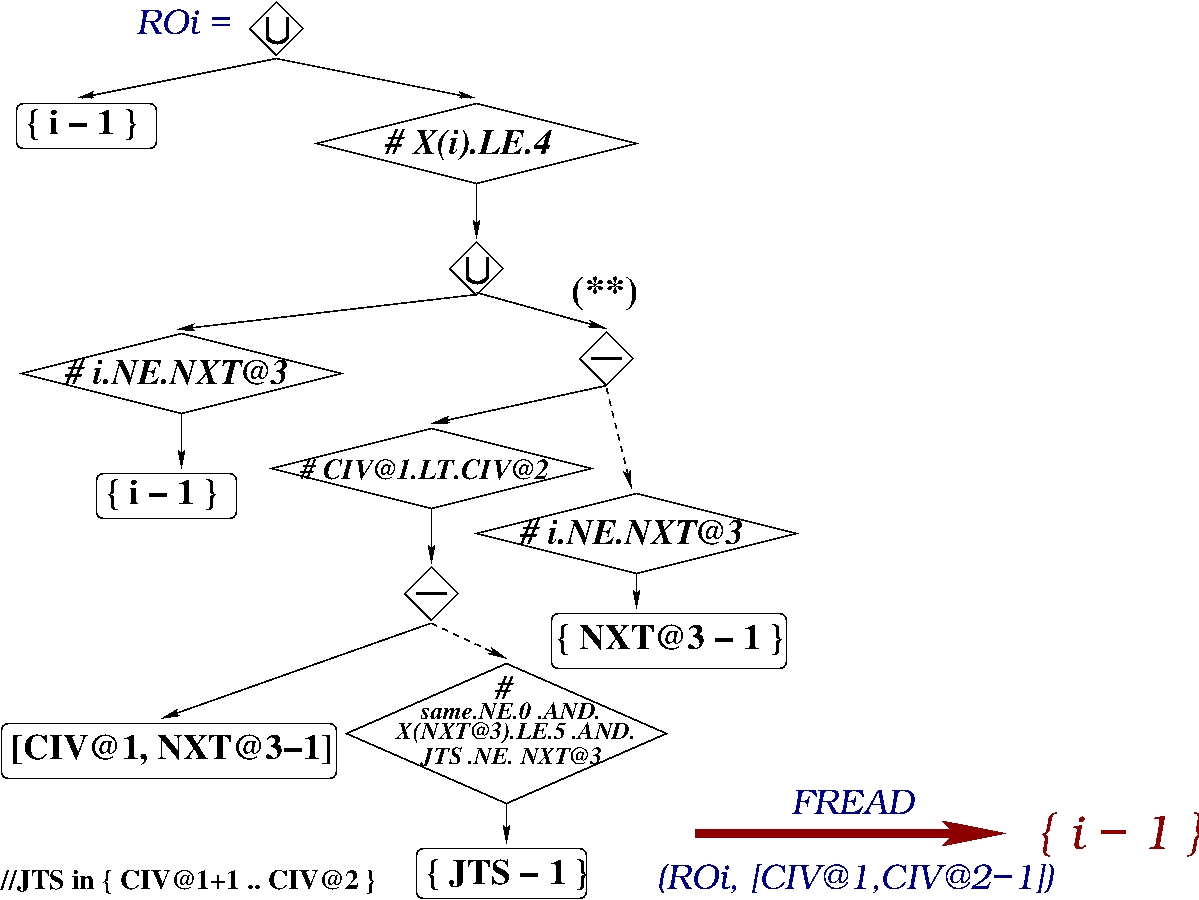
\includegraphics[width=.38\textwidth]{\Figures/ROio_USR_EXTEND_do500.jpg}
	  	}
	} & {  \hspace{-22ex}
		\subfigure[$\mbox{~}$]{
          	\label{fig:VegEXTEND} 
			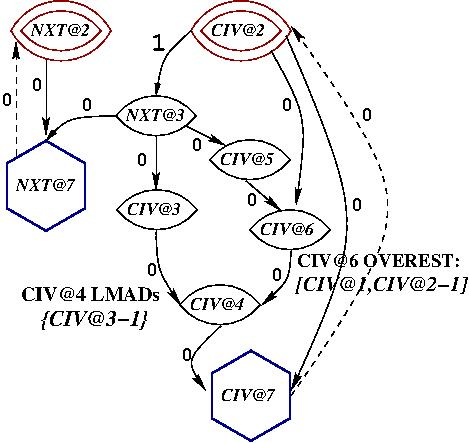
\includegraphics[width=.23\textwidth]{\Figures/VEG_EXTEND.jpg}
	  	}
	}
    \end{tabular} \vspace{15ex} 
\vspace{-7ex}
\caption{(a) {\sc ro}$_i$ {\sc usr} \& (b) {\tt civ}'s {\sc veg} for {\tt EXTEND\_do500}.} 
\label{fig:Track} %
\end{figure}
  
\vspace{1ex}

{\bf 1. External Variables Allowed in VEG.}
%
Sometimes two different variables are semantically the same {\sc civ},
for example in the sequence {\tt nxt=civ;$\ldots$nxt=nxt+1;$\ldots$civ=nxt},
shown in the {\sc veg} graph of Figure~\ref{fig:VegEXTEND}. 
It follows that we allow (external) variables such as {\tt nxt@3} to belong to
the {\sc veg} graph of {\tt civ} because (i) they semantically contribute to 
the flow of {\tt civ} values and (ii) the extended {\sc veg} still complies 
with the definition of a {\sc civ} variable (see Section~\ref{subsec:Background}), 
and because (iii) subscripts may contain both variables.  

The analysis treats {\tt nxt@3} as any other member of the {\tt civ} family of 
variables, except that summaries {\em cannot} be associated with external nodes,
because the latter do not necessarily encapsulate the correct control flow,
i.e., the $\gamma$ nodes of variable {\tt nxt} are not part of {\tt civ}'s {\sc veg} graph.

\vspace{1ex}

{\bf 2. Filtering The Read Set}. The {\sc ro} ({\sc usr}) summary corresponding 
to iteration {\tt i} of loop {\tt EXTEND\_do500} is shown in 
Figure~\ref{fig:USR_ROio_EXTEND_do500}, where $\cup$, $-$ and $\#$ internal nodes 
correspond to set union, subtraction and gates, respectively.   
One can observe that {\sc ro}$_{i}$ is already nontrivial, and using it as
input to outer-level summarization would result in complex set expressions,
which would be ill-suited for computing independence.
%
We use instead a filtering technique based on the observation that
the contribution of {\sc ro}$_i$ to the loop-aggregated
{\sc ro} set cannot possibly belong to $\cup_{k=1}^{i-1}${\sc wf}$_k$.
The same property holds for the read-write set.

\begin{figure}[t]
\begin{scriptsize}
USR {\bf FREAD}($R$ : USR, $WF^p$ : LMAD) \vspace{1ex} \newline
$\mbox{ }\mbox{ }$// {\bf {\em Output:}} $R$ filtered-out of $WF^p$ terms. \vspace{1ex} \newline
$\mbox{ }\mbox{ }$Case $R$ of: \vspace{1ex} \newline
$\mbox{ }\mbox{ }\mbox{ }\mbox{ }$ LMAD $L$:  
{\bf IF} $\mathcal{F}(L - WF^p)$ {\bf THEN} $\emptyset$ {\bf ELSE} $L$ \vspace{1ex} \newline
$\mbox{ }\mbox{ }\mbox{ }\mbox{ }$ $g\#A$: $g\#${\bf FREAD}($A$,$WF^p$)  \vspace{1ex} \newline   
$\mbox{ }\mbox{ }\mbox{ }\mbox{ }$ $A \cup B$: {\bf FREAD}($A$,$WF^p$) $\cup$ {\bf FREAD}($B$,$WF^p$) \vspace{1ex} \newline
$\mbox{ }\mbox{ }\mbox{ }\mbox{ }$ $A \cap B$: {\bf FREAD}($A$,$WF^p$) $\cap$ {\bf FREAD}($B$,$WF^p$) \vspace{1ex} \newline
$\mbox{ }\mbox{ }\mbox{ }\mbox{ }$ $A - B$: {\bf FREAD}($A$,$\lfloor B \rfloor \cup WF^p$)   \vspace{1ex} \newline
$\mbox{ }\mbox{ }\mbox{ }\mbox{ }$ LOOP OR CALLSITE :   \vspace{1ex} \newline   
$\mbox{ }\mbox{ }\mbox{ }$ 
$\mbox{ }\mbox{ }\mbox{ }$ 
          {\bf IF}($\mathcal{F}$($\lceil R \rceil - WF^p$) THEN $\emptyset$ ELSE $R$
\end{scriptsize}
\caption{ Read-Set Filtering Algorithm.}
\label{fig:ReadFilt} %
\end{figure}
 

Figure~\ref{fig:ReadFilt} shows the recursively-defined operator {\tt FREAD} that
filters out from the {\sc ro}$_i$ ({\sc rw}$_i$) set, the terms that are included 
into an interval underestimate of $\lfloor\cup_{k=1}^{i-1}${\sc wf}$_k\rfloor$, 
denoted $WF^p$.
The result summary replaces {\sc ro}$_i$ in Figure~\ref{fig:LoopAggreg}'s equations.
%
The algorithm pattern-matches the shape of the read-only summary:
If the current node is an interval $L$ then we extract a % of {\sc ro}$_i$ 
sufficient predicate for $L - WF^p = \emptyset$ by using the {\sc usr}-to-predicate
translation $\mathcal{F}$ mentioned in Section~\ref{subsec:Background}.   
If the predicate is statically {\tt true}  then $L$ is filtered out, 
otherwise $L$ (or $L-WF^p$) is kept.

Similarly, if the current node, named $R$, is a loop or callsite node, 
then we check using $\mathcal{F}$ whether an interval overestimate of 
$R$ is included in $WF^p$; if so then $R$ is filtered out, otherwise 
it is kept.  
%
If $R$ is a gate or union or intersection node,
then each term is filtered and the results are composed back. 
%
If $R$ is a subtraction node $A-B$ then $A$ is filtered with the union 
of $WF^p$ and an interval underestimate of $B$. 

Filtering the read-only set depicted in Figure~\ref{fig:USR_ROio_EXTEND_do500}
with the computed $\lfloor \cup_{k=1}^{i-1}WF_k\rfloor=${\tt[civ@1,civ@2-1]}
results in the simple $RO'_{i} = {\tt\{i-1\}}$, where the problematic 
subtraction node, denoted by {\tt (**)} in Figure, was simplified\footnote{
The algorithm has used the {\sc veg}-derived properties {\tt civ@1$<$jts$\leq$civ@2} 
and {\tt M$\leq$civ@1}, where {\tt civ@1} is the {\sc civ} value 
just before entering the loop, and {\tt M} is the loop upper bound. Since 
{\tt civ}-values are monotonically increasing, it also follows: 
{\tt i $\leq$ M $\leq$ civ@1 $\leq$ civ@2 $<$ nxt@3.}
}
to $\emptyset$.%Similarly $RW'_{i} = \emptyset$.


\vspace{1ex}

{\bf 3. Output-Dependence Pattern.} 
%
When a {\sc civ} subscript is written on a {\tt 0}-evolution path,
then cross-iteration dependencies are likely to occur because 
the next writing iteration is likely to overwrite the same subscripts.
This section demonstrates on loop {\tt EXTEND\_do400}
a technique that can resolve mostly statically such dependencies.
%
Assume we have per-iteration and partial-recurrence {\sc wf} 
sets of shape:\vspace{1ex}\\
\noindent$\lceil WF_i\rceil${\tt=[civ@1,civ@8~~]},
$\lceil\cup_{k=1}^{i-1}WF_{k} \rceil${\tt=[civ,civ@1]},\\
\noindent$\lfloor WF_i\rfloor${\tt=[civ@1,civ@8-1]},
$\lfloor\cup_{k=1}^{i-1}WF_k \rfloor${\tt=[civ,civ@1-1]}\vspace{1ex}\\
where {\tt civ@1} and {\tt civ@8} are the $\mu$ and back nodes of
the {\sc veg} associated to loop {\tt EXTEND\_do400} and variable {\tt civ}.
%
One can observe that output-dependencies may exist, since
the output-independence equation of Figure~\ref{fig:IndEq} is not satisfied:
$\lceil WF_{i}\rceil \cap \lceil \cup_{k=1}^{i-1}WF_{k} \rceil \equiv {\tt\{civ@1\}}\ne\emptyset$.

Still, dependencies exhibit a well-structured pattern that our 
implementation exploits. The key observations are: 
\begin{itemize}
    \item Indices belonging to $\lfloor{}WF_{j}\rfloor$ underestimate  
            do not result in cross dependencies:
        $\lfloor WF_{i}\rfloor\mbox{~}\cap\mbox{~}\cup_{k=1}^{i-1}\lfloor WF_{k}\rfloor~=~\emptyset$.

    \item All remaining indices, 
        $\lceil WF_{i}\rceil - \lfloor WF_{i}\rfloor = {\tt\{civ@8\}}$,
        are overwritten by the next {\sc civ}-increasing iteration:
        {\tt{}civ@8>civ@1} $\Rightarrow$
        {\tt\{civ@1\}} $\subseteq\lfloor WF_{i}\rfloor${\tt=[civ@1,civ@8-1]}
        %
        where {\tt\{civ@8\}} of the previous iteration was rewritten as 
        {\tt\{civ@1\}} of the next {\sc civ}-increasing iteration.

    \item Last iteration increases the {\sc civ} value; this 
        holds for {\tt EXTEND\_do400} because {\sc civ} is 
        updated in an inner loop.
\end{itemize}

If all properties hold, then the output-dependency pattern is resolved 
by privatizing the array (updates) and by copying out, at 
iteration's end, the indices belonging to the $\lfloor WF_i\rfloor$ 
{\em underestimate}, i.e., {\tt[civ@1,civ@8-1]}.
The last iteration copies in and out the overestimate (or updates directly),
and because it increases {\sc civ}, it is guaranteed to overwrite the 
uncommitted part of previous (non-increasing) iterations.
%
The last property requires runtime verification, during the {\sc civ}-value
(pre)computation, while the first two are derived statically for the current 
loop, but in general, they may also use runtime verification.

%\vspace{1ex}
%{\bf 4. Privatizable Stack.} Our analysis also extends (with
%some modifications) to a stack-like access pattern in which
%the {\sc civ} values are only piecewise monotonic.
%This is discusses in Appendix~\ref{sec:Stack} in the
%context of loop {\tt ACCEL\_do10} from {\tt tree} benchmark
%that exhibits a privatizable stack. 

\enlargethispage{\baselineskip}

% : Beyond Monotonicity 
\subsection{Privatizing Stack-Like Accesses} 
\label{sec:Stack}

While we have studied so far the case when the {\sc civ} evolution
throughout a loop is monotonic, this section investigates a stack-like 
access pattern that can still be solved in a similar fashion, by 
studying monotonicity piecewise.
 
For example, the code in Figure~\ref{fig:Tree}(a) is a simplified
version of loop {\tt ACCEL\_do10} from {\tt tree} benchmark. 
Each iteration of the outer loop maintains its own
stack, denoted {\tt X}, that is used in the {\tt while} loop to 
compute a result {\tt res}:
The {\tt while} loop is exited when the stack is empty, and each
iteration pops one element and, later on, pushes
up-to-eight new elements from/to the stack. 

The goal is to prove that the stack {\tt X} is privatizable in the
context of the outer loop.   The plan is to devise an analysis
capable of overestimating the {\em disjoint intervals} of the
{\tt while}-loop-aggregated (i) {\em read set}, i.e., 
{\sc r}$=${\sc ro}$~\cup~${\sc rw}, and (ii) {\em write-first set}. 
In our case, this would result in  
$\lceil${\sc r}$\rceil=${\tt[0,civ-1]}, and
$\lceil${\sc wf}$\rceil=${\tt[civ,SS]}, where {\tt SS} denotes
the stack size and  {\tt civ} is the value before entering the 
{\tt while} loop, i.e., $1$.  

One can now observe that the read set of the {\tt while} loop 
is included in the {\sc wf} set of the region just before the 
{\tt while} loop, i.e., {\tt \{0\} $\subseteq$ \{0\}}, due to the 
first update to {\tt X(civ)}. It follows that the read set of
each iteration of the outer loop is the empty set, 
hence {\tt X} can be safely privatized. 


\begin{figure}
\begin{minipage}{0.4\columnwidth}
\begin{colorcode}
DO i = 1, N, 1
 civ = 1
 {\bf{}X}(civ) =...
 WHILE ( civ.GT.0 )
  civ@2=\mymath{\gamma}(civ,civ@5)
  q = {\bf X}(civ@2)
  civ@3 = civ@2 - 1
  IF (q.LE.5) THEN
   res = res +..q..
  ELSE
   DO j = 1, 8, 1
    IF (civ.LT.SIZE) 
      civ = civ + 1
      {\bf{}X}(civ)=...
   ENDIF ENDDO
   civ@9=\mymath{\gamma}(civ@3,..)
  ENDIF
  civ@5=\mymath{\gamma}(civ@3,civ@9)
ENDWHILE ENDDO   
\end{colorcode}
\vspace{-1ex}
(a) Loop {\tt ACCEL\_do10}.
\end{minipage}
\begin{minipage}{0.56\columnwidth}
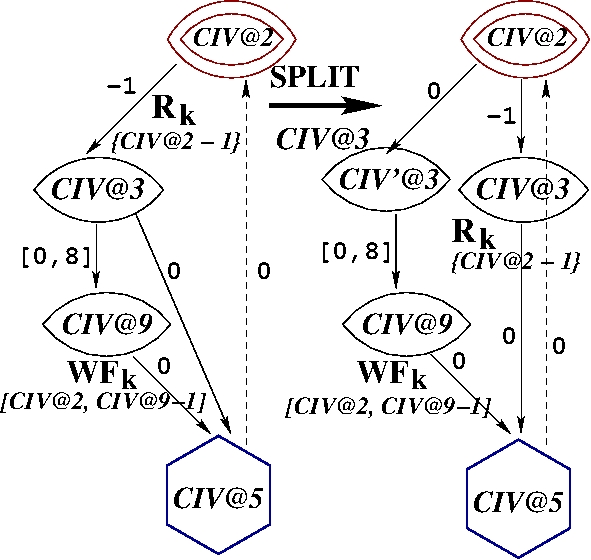
\includegraphics[width=1.1\textwidth]{\Figures/VEG_TREE.jpg}\\
$\mbox{ }\mbox{ }\mbox{ }\mbox{ }\mbox{ }\mbox{ }\mbox{ }$(b) Original \& Spliced {\sc veg}s.
\end{minipage}
\caption{a) Stack-like access in benchmark {\tt tree} and (b) the {\sc veg} graphs of the while loop.}
\vspace{-1ex}
\label{fig:Tree} %
\end{figure}


The original {\sc veg} of the {\tt while} loop, depicted on the left 
side of Figure~\ref{fig:Tree}(b), exhibits a non-monotonic {\sc civ}$_\mu$
evolution, i.e., it can be anywhere between minus one and seven.
%
The intuition is to use an inductive summarization for the read and {\sc wf} sets:
{\em The base case} corresponds to analyzing the first iteration to determine a split point, 
denoted {\tt SP}, from which, without loss of generality, the write-first set increases in the 
upper-bound direction, i.e., {\sc wf}{\tt=[SP,$\ldots$]}, and the read set increases 
in the lower-bound direction, i.e., {\sc r}{\tt=[$\ldots$,SP-1]}, where we 
have assumed for simplicity the stride to be {\tt 1}.
(The other case is treated in a similar fashion.)

With our example, {\sc wf}$_k=${\tt (q.GT.5)\#[civ@2,civ@9-1]}
is associated with {\sc veg} node {\tt civ@9}, and 
{\sc r}$_k=${\tt \{civ@2-1\}}, as before, with {\tt civ@3}, 
where $k$ denotes an arbitrary iteration of the {\tt while} loop.
The split point is {\tt SP=civ=1}, since {\tt civ@2} equals {\tt civ} 
for the first iteration.

{\em The second step} is to attempt a semantics-preserving {\sc veg} transformation
such that (i) each {\sc civ}-decreasing/increasing path holds only intervals 
belonging to the read/{\sc wf} set, respectively, and (ii) a $0$-path holds
only empty intervals.

The semantics to be preserved is that the aggregated-read/{\sc wf} summaries of
any valid execution of the original {\sc veg} should be preserved by (at least) 
one valid execution of the transformed {\sc veg}.  The approach is
to search for a path where, for example,  the read set occurs before a {\sc wf} set.
One can then splice a convenient node {\sc civ}$_{sp}$ between the two, and 
introduce a $0$-evolution path from {\sc civ}$_{sp}$ to the back node, 
if none already exist,
and a $0$-evolution path from {\sc civ}$_\mu$ to the spliced node {\sc civ}$_{sp}^{cl}$.
The original path is translated with the original path up to {\sc civ}$_{sp}$,
then directly to the back node, followed by the $0$-evolution path to  
{\sc civ}$_{sp}^{cl}$, and the rest of the original path. The process is
repeated to a fix-point.

For example, the right side of Figure~\ref{fig:Tree}(b) shows the result of
splitting  node {\tt civ@3} of the original {\sc veg}: a new $0$-evolution
edge now connects {\tt civ@2} and {\tt civ'@3}. In addition, the {\sc wf} set 
has been adjusted to the new {\sc civ}$_\mu$ value, but has also
been conservatively extended with the result of the read-set of the previous
(transformed) iteration, resulting in the same $WF_k$ interval as 
in the original {\sc veg}. 



{\em Finally, the third step} is to aggregate the {\sc wf} and read sets 
only on the monotonically increasing and decreasing (including $0$) paths,
respectively. 
If the read and {\sc wf} results are exact, i.e., the under 
and overestimate are identical, and have shapes {\tt[$\ldots$,SP-1]}  
and {\tt[SP,$\ldots$]}, respectively, then 
one can prove that the result of this piecewise monotonic
aggregation matches the result of the original-{\tt while} aggregation:
a read-set overestimate is {\tt [0,SP-1]}, and privatization was proven.
%Note that the lower bound can be improved by using the {\tt while}-stop condition.

\subsection{The CIV Slice}
\label{subsect:CivImplem}

The independence results discussed in previous sections have referred 
so far to disambiguating array accesses that exhibit {\sc civ} 
subscripts, but not to the computation of the {\sc civ} values.
%
When the {\sc civ} variable is not privatisable in the context of the 
target loop, e.g., in Figure~\ref{fig:codeActforCorrec}(a), 
the {\sc civ} is the source of cross-iteration flow dependencies: 
it is always updated in reduction-like statements, e.g., {\tt civ=civ+3*C(i)},
but it is read in arbitrary statements, e.g., in a subscript.

While related approaches~\cite{PaduaDemDrInterproc,VEG} avoid this, we always pre-compute in
parallel, prior to loop execution, the {\sc civ}$_\mu$ values at the beginning 
of each (chunk of) iteration(s).
Reasons are threefold: {\em First}, in most cases 
the runtime overhead is small. {\em Second}, the {\sc civ} values may dictate
whether the loop is independent or not: For example,  the flow-independence
predicate of the loop in Figure~\ref{fig:codeActforCorrec}(a), 
${\tt N} \le {\tt Q}~\vee~{\tt civ@5} < {\tt M}$,
depends on {\tt civ@5}, and resolving statically the output 
dependencies of {\tt EXTEND\_do400}, depends, as
per Section~\ref{subsec:Track}, on establishing whether the last
iteration has increased the {\sc civ} value. 
%
{\em Third}, {\sc civ} values may flow in the computation
of data (rather than only subscripts), e.g., the recurrent
formula of the Sobol random number generator, used in
benchmark {\tt Pricing}  of Section~\ref{sec:EmpEval}.

{\sc civ}$_\mu$ values are (pre)computed by extracting the loop-slice
that contains the transitive closure of all statements 
that are necessary to compute the {\sc civ} variable
(we use the control-dependency graph). 
We privatize all arrays and scalars, including {\sc civ}, that are not 
read-only inside the slice, where each iteration copies-in the  indices 
of its $RO_i \cup RW_i$ set. Finally, an iteration-header statement is 
inserted to initialize {\sc civ} to the value just before the loop ({\tt Q}), 
and similarly, the end-of-iteration value minus {\tt Q} is saved into array 
{\tt CIVS}.  


\begin{figure*}
\begin{minipage}{1.0\columnwidth}
\begin{colorcode}
//\mymath{slice for computing partial civ values}
DOALL i = M, N, 1      \$PRIVATIZED(civ,i)
  civ = Q
  IF ( C(i) .GT. 0 ) civ = civ + 3*C(i)
  CIVS(i-M+1) = civ - Q
ENDDOALL

//\mymath{SCAN(op{\tt{}+},e,n,{\tt{}X})\equiv}\{\mymath{e},\mymath{e}+X(1),..,\mymath{e}+X(1)+..+X(n)\}
SCAN(op +, Q, N-M+1, CIVS)

//\mymath{civ values are plugged in the loop} 
DOALL i = M, N, 1      \$PRIVATIZED(civ,i)
  civ = CIVS(i-M+1)
  ... \mymath{rest of the loop code} 
ENDDOALL
                (a)
\end{colorcode}
\end{minipage}
%
\begin{minipage}{1.02\columnwidth}
\centering
\scriptsize   
\begin{tabular}{|c|l|l|c|c|l|} \hline
\multicolumn{6}{|c|}{Properties of Benchmarks Exhibiting Important Loops That Use {\sc civ}s} \\ \hline
{\sc bench} & {\sc properties} & {\sc do loop}  & {\sc lsc}\%  & T$_{P/S}^L$(s) & {\sc type} \\ \hline
{\sc bdna}  &  T$_{P/S}$=.19/.65 s         & {\sc actfor\_500}  & 47.8 & .05/.31 & {\sc st-par}     \\ 
{\tt P=8}         &  {\sc sc}=87\%,{\sc ov}=0\%  & {\sc actfor\_240}  & 35.6 & .04/.23 & {\sc civ}$_{\tt{}AGG}$    \\ \hline 
             &  T$_{P/S}$=1.14/3.1 s         & {\sc gmttst\_120}  & 17.4 & .27/.54 & {\sc {\sc fi} {\sc o(1)}}   \\ 
{\sc nasa7}  &  {\sc sc}=98\%,{\sc ov}=0\%  & {\sc emit\_5}      & 13.6 & .09/.42 & {\sc civ}$_{\tt{}COMP}$   \\  % ,{\sc oi} {\sc o(n)}
{\tt P=8}        &                              &                      &                & & {\sc oi} {\sc o(n)}       \\
             &                              & {\sc btrtst\_120}  & 10.1 & .05/.31 & {\sc fi} {\sc o(1)}        \\ \hline
{\sc track}  &  T$_{P/S}$=6.6/16.8 s         & {\sc fptrak\_300}  & 52.8 & 3.6/8.9 & {\sc civ}$_{\tt{}COMP}$   \\ 
{\tt P=8}        &  {\sc sc}=97\%,{\sc ov}=45\%  & {\sc extend\_400}  & 43.9 & 2.3/7.4 & {\sc civ}$_{\tt{}COMP}$ \\ \hline 
{\sc tree}   &  T$_{P/S}$=12.8/59 s        & {\sc accel\_10}    & 91.2 & 7.6/54 & {\sc civ}$_{\tt{}AGG}$  \\            %58.6%53.5
{\tt P=8}        &  {\sc sc}=91\%,{\sc ov}=0\% &                    &      &          &                           \\ \hline 
{\sc price\_i} &  T$_{P/S}$=.29/2.0 s        & {\sc price\_i\_10} & 99   & .29/2.0  & {\sc civ}$_{\tt{}AGG}$ \\ 
{\tt P=8}          &  {\sc sc}=99\%,{\sc ov}=0\% &                    &      &          &                           \\ \hline 
{\sc price\_r} &  T$_{P/S}$=.17/.98 s          & {\sc price\_r\_10}& 99   & .17/.98  & {\sc civ}$_{\tt{}COMP}$ \\ 

{\tt P=8}          &  {\sc sc}=99\%,{\sc ov}=6.4\% &                  &      &          &                          \\ \hline 
\end{tabular}
\begin{colorcode}

                        (b)
\end{colorcode}
\end{minipage}
\caption{ (a) Parallel Computation of {\sc civ}$_\mu$ Values.     (b) Characterization of Important CIV Loops.}
\label{fig:CivSlice} %
\end{figure*}

%For example, 
Figure~\ref{fig:CivSlice}(a) shows the {\sc civ} slice of the loop
in Figure~\ref{fig:codeActforCorrec}(a), where scalars {\tt i} and {\tt civ}
were privatized. The slice computes the per-iteration {\sc civ} increments 
and records them in {\tt CIVS}. Then {\tt SCAN}
computes in parallel the prefix sum of the {\tt CIVS} values, 
which are used each by one iteration of the parallelized loop.
%
Correctness requirements are {\em twofold}:  

{\em First}, all symbols that appear in the slice have been already proven 
to not introduce cross-iteration dependencies in the original loop; otherwise 
the computation of the slice might violate the semantics of the sequential execution. 

{\em Second}, {\sc civ} variables may appear in the slice only in reduction-like statements, 
such as {\tt civ=civ+1}.
If this holds than the final {\sc civ} value would correspond to an (additive) reduction, 
and hence, the intermediate {\sc civ}$_\mu$ values are safely computed via the parallel 
prefix sum of the values in {\tt CIVS}. 

If the latter does not hold,  
then we have a cycle between {\sc civ}-value computation and their use.   
We address such a case via a fixed-point implementation,
which (i) optimistically computes the {\sc civ} values as before, and then (ii) logically 
re-executes the slice on the computed-{\sc civ} values and checks (in parallel) 
whether the resulted value matches the input-value of the next iteration. 
%
If the check succeeds across all iterations, one can prove correctness by induction:
The first iteration is always correct. If the value at the end of the first iteration 
coincides with the input of the second, then the second iteration 
is correct, etc.  

\enlargethispage{\baselineskip}

Finally, {\sc civ}$_\mu$ input values are plugged in the 
parallel execution of the original loop: The arrays that were proven flow and output
independent are shared, i.e., not privatized.   For cases such as {\tt EXTEND\_do400},
that exhibit the special pattern of output dependencies, we adopt a strategy similar
to the one used for {\sc civ} computation: arrays such as {\tt X} are privatized,
their read-set {\sc ro}$_i$ $\cup$ {\sc rw}$_i$ is copied in, and the per-iteration 
{\sc wf} underestimate
is copied-out at the iteration's end.   Our technique is deeply integrated with the
underlying compiler framework: On the one hand, $\mathcal{F}$ uses the {\sc civ}-summarized
over and underestimates to derive sufficient-independence predicates.
%
On the other hand $\mathcal{F}$ is used in the summarization process, for example 
to simplify the {\sc ro}/{\sc rw} per-iteration sets, and thus to optimize the 
size of the data that needs to be copied in.  Similarly, Fourier-Motzkin-like
elimination reduces both loop indices and {\sc civ}s, i.e., when {\sc civ}'s 
bounds are derivable from its {\sc veg}.



\section{Experimental Evaluation}
\label{sec:EmpEval}

While we have analyzed~\cite{CosPLDI} more than two thousand loops from about thirty 
benchmarks ({\sc spec}, {\sc PerfectClub} and more recent ones~\cite{LexiFiPricing}), 
this section reports only five benchmarks in which our {\sc civ} analysis was crucial 
for efficient benchmark-level parallelization: we consider only 
{\sc civ} loops that have a significant global coverage and belong to the most
beneficial schedule of parallelized loops.   However, the number
of loops exhibiting {\sc civ} subscripts is much larger, and we believe
it is significant that $17\%$ (5 out of 30) of the analyzed benchmarks contain 
essential {\sc civ} loops. 

%We evaluate our technique on a number of benchmarks containing loops that cover a significant
%fraction of the total sequential runtime and that exhibit {\sc civ}-based accesses.
%
Figure~\ref{fig:CivSlice}(b) characterizes several representative loops, named in 
the third column, and their corresponding benchmarks, named in the first column.
The reported parallel runtime were measured on {\tt P=8} cores.


The second column shows 
(i)   the parallel and sequential runtime, T$_{P/S}$, measured in seconds,
(ii)  the percentage, {\sc sc}, of the sequential runtime that has been parallelized, and 
(iii) the overhead of the associated runtime tests, if any, which is represented as percentage of
        the total-parallel runtime. With our benchmarks, the only runtime test that introduces
        non-negligible overhead is the (pre)computation of {\sc civ} values, 
        denoted {\sc civ}$_{\tt{}COMP}$, and presented in Section~\ref{subsect:CivImplem}.   


\begin{figure*}[t] 
\begin{minipage}{1.2\columnwidth}
    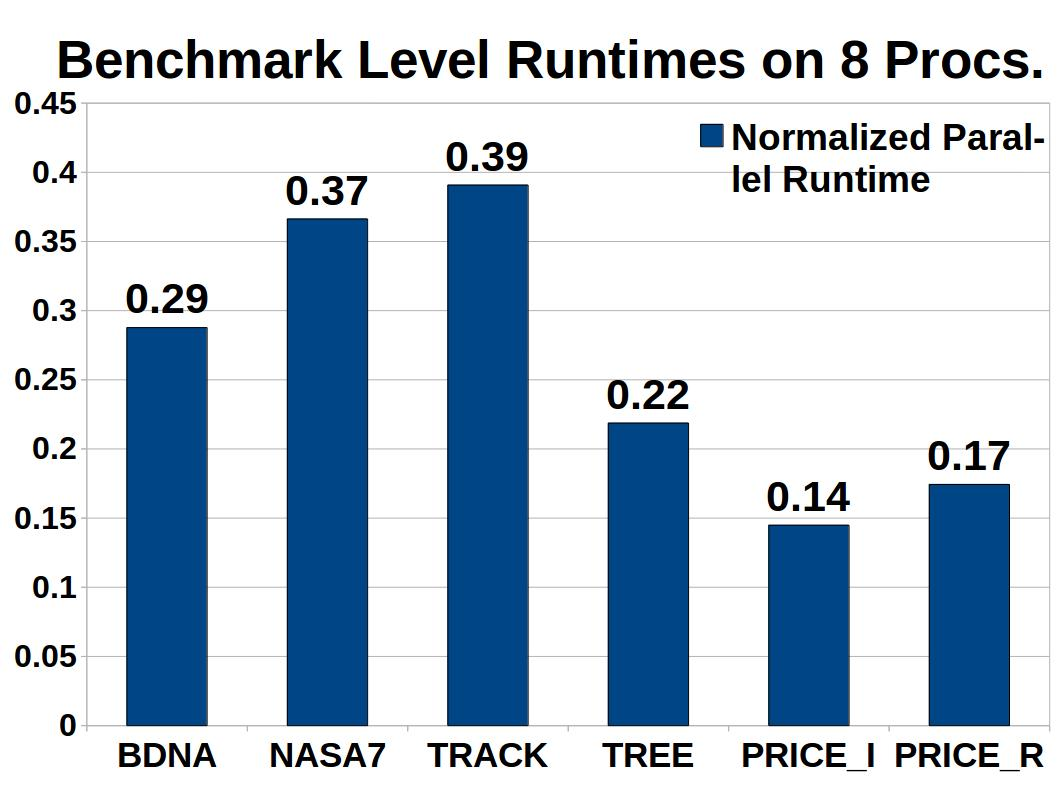
\includegraphics[width=0.55\textwidth]{\Figures/EmpRes/BenchParRes.jpg} 

      {\bf~~~~~~~~~~~~~~~~~~~~~~~~~~~~~(a)} \vspace{2ex}

    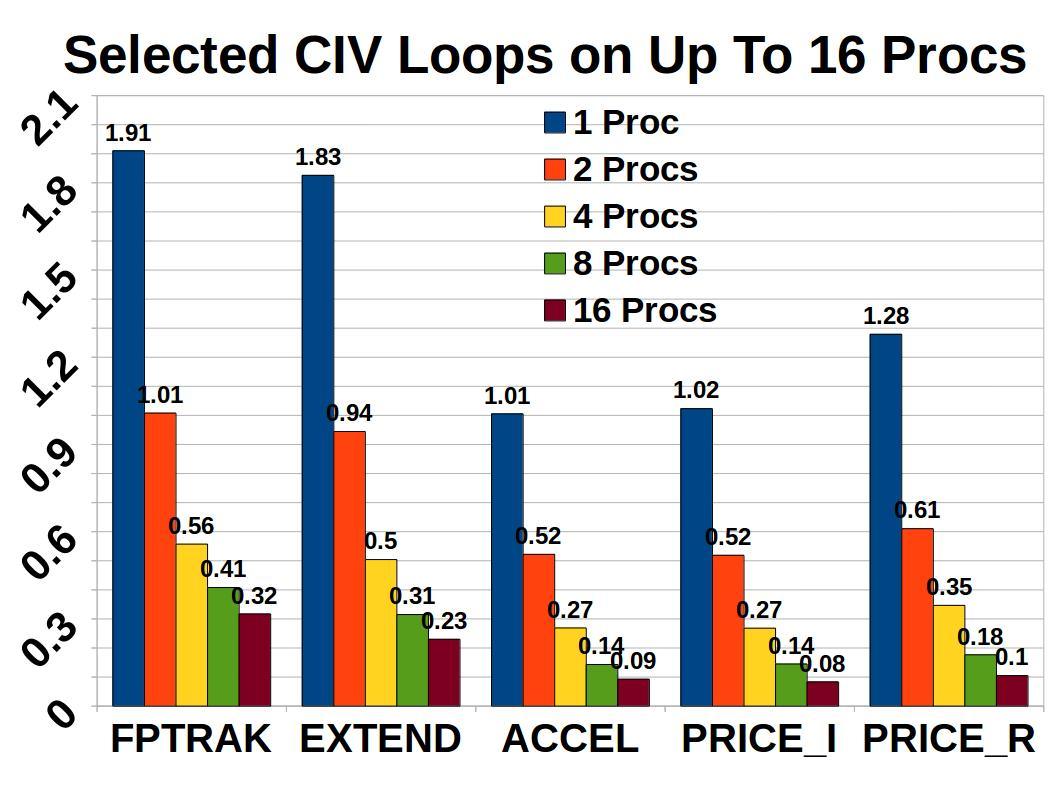
\includegraphics[width=0.55\textwidth]{\Figures/EmpRes/LoopScalRes.jpg}
      
      {\bf~~~~~~~~~~~~~~~~~~~~~~~~~~~~~(c)}\vspace{1ex}

\end{minipage}
\begin{minipage}{0.9\columnwidth}
    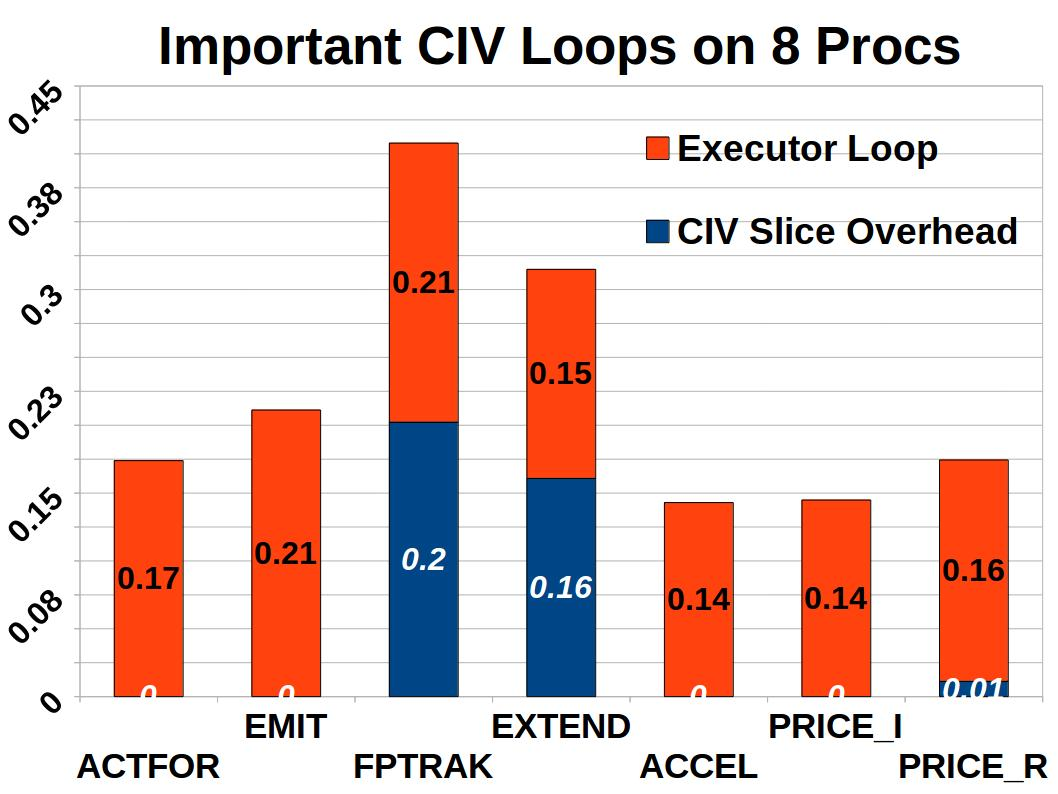
\includegraphics[width=0.75\textwidth]{\Figures/EmpRes/LoopParRes.jpg} 

      {\bf~~~~~~~~~~~~~~~~~~~~~~~~~~~~~(b)}\vspace{2ex}

   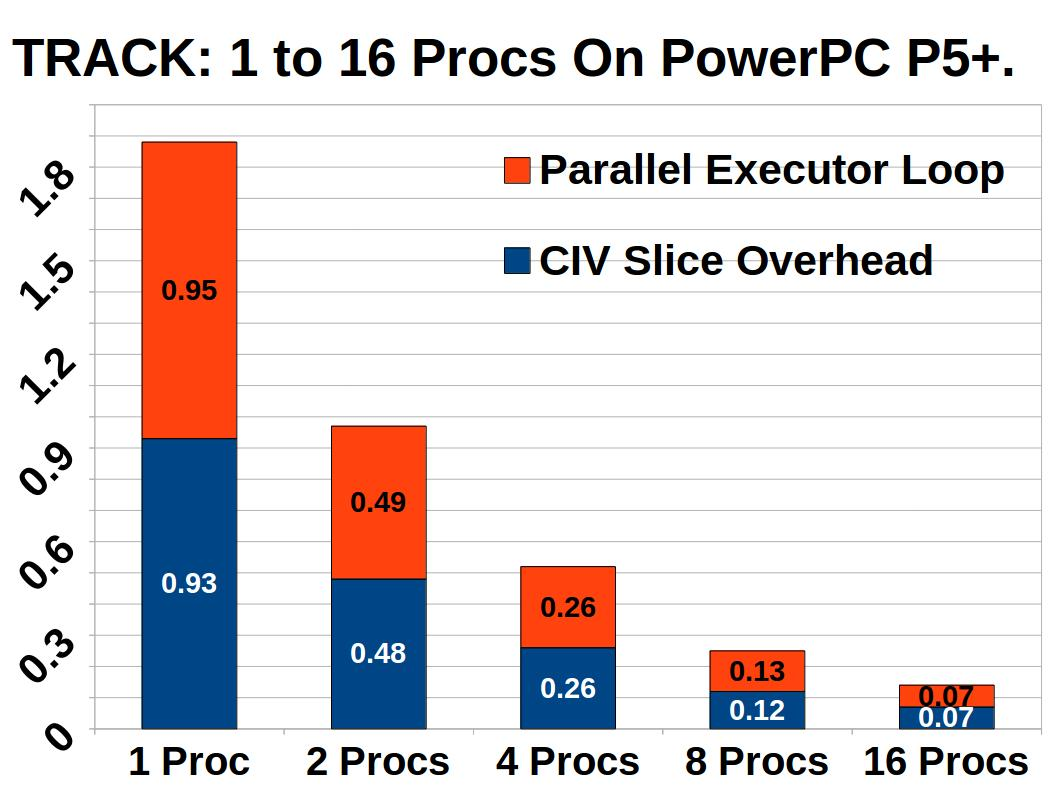
\includegraphics[width=0.75\textwidth]{\Figures/EmpRes/TrackScal.jpg}
      
      {\bf~~~~~~~~~~~~~~~~~~~~~~~~~~~~~(d)}\vspace{1ex}

\end{minipage}
\caption{ Benchmark and Loop-Level Normalized (Total) Parallel Runtime. Sequential Runtime is 1.}
\label{fig:ParRuntime} %
\end{figure*}


The third column shows the names of the most important loops,
the fourth shows their sequential coverage, {\sc lsc}, and the
fifth shows each loop's parallel and sequential runtime, T$_{P/S}^L$, in seconds.
%
We note that benchmarks {\tt bdna} and {\tt nasa7} have poor scalability, e.g., very small
performance gain from four to eight-core execution, because they exhibit
small (historical) datasets: low-granularity important loops that limits the 
profitability of parallelization.
In addition, (i) loop {\tt GMTTST\_do120} 
is parallel but has loop-count three, and (ii) loop {\tt RESTAR\_do15},
which covers $9.3\%$ of the sequential runtime, uses {\sc io} operations,
and was run sequentially. 

The sixth column shows {\em how} the loop was classified parallel: {\sc fi} {\sc o(1)}
means that a predicate of runtime complexity {\sc o(1)} has validated loop's flow
independence at runtime. {\sc civ}$_{\tt{}AGG}$ indicates that {\sc civ}-based summarization 
was instrumental in proving independence statically, and {\sc civ}$_{\tt{}COMP}$ means that,
in addition to {\sc civ}$_{\tt{}AGG}$, the {\sc civ}$_\mu$ values were precomputed
at runtime, i.e., {\sc civ} was not privatizable.  {\sc st-par} indicates static
parallelization of a ``regular'' loop. 


\vspace{1ex}

{\bf Our Test Suite} consists of benchmarks {\tt bdna} and {\tt track} 
from {\sc perfect-club} suite: (i) {\tt ACTFOR\_do240} is a {\sc civ} loop
that uses a vector in which elements are inserted at the end, and
both the {\sc civ} and the vector array can be privatized, (ii) 
loop {\tt FPTRAK\_do300} from {\tt track} is similar to {\tt EXTEND\_do400},
and loop {\tt CORREC\_do401} is not shown because 
its sequential coverage is under $1\%$. 
%
Benchmark {\tt nasa7} is part of {\sc spec2000} suite, and its loop {\tt EMIT\_do5}
is similar to {\tt ACTFOR\_do240} except that output and flow independence 
is proven with runtime predicates, and it also requires precomputation of {\sc civ} values.
%
Benchmark {\tt tree}~\cite{Treecode} is an implementation of the Barnes-Hut algorithm.
Its main loop, {\tt ACCEL\_do10}, exhibits the stack-access pattern of Figure~\ref{fig:Tree}(a),
and accounts for $91\%$ of the sequential runtime. The remaining $9\%$ corresponds to {\sc io}
operations and cannot be parallelized.
%
Finally,  {\tt price\_i/r} is a (simplified) kernel of a real-world application that
computes the price of a financial contract~\cite{LexiFiPricing}:   The difference
between the two versions is that (i) {\tt price\_i} uses an independent Sobol-random-number-generator
algorithm, i.e., computing the $i^{th}$ random number requires only the value of $i$,
and exhibits a {\sc civ} pattern similar with {\tt ACTFOR\_do240}, 
while (ii) {\tt price\_r} uses a faster, recurrent formula that computes the 
$i^{th}$ random number based on the previous $(i-1)^{th}$ one. 
This means that in {\tt price\_r} the {\sc civ} is not used for indexing
but directly in the computation of Sobol numbers, i.e., a parallel prefix 
scan with exclusive-or operator {\tt xor}. 
Parallelization of {\tt price\_r} consists of (pre)computing
in parallel these {\sc civ}$_\mu$ values, in the manner of 
Section~\ref{subsect:CivImplem}.   
%
Because our implementation does not support {\tt xor},
we have manually turned the {\tt xor} into addition before 
compilation and then back to {\tt xor} after compilation. 

\vspace{1ex}

{\bf Experimental Methodology.} Our source-to-source compiler receives as
input a sequential {\tt Fortran77} program and automatically analysis loop-level 
parallelism and produces {\tt OpenMP} code.  The sequential and parallel 
code were compiled with {\tt gfortran}, option {\tt -O3}, and were run on 
a $16$-core {\tt AMD Opteron(TM) 6274} system with $128${\tt GB} memory. 

\vspace{1ex}

{\bf Results.} Figure~\ref{fig:ParRuntime}(a)~and~(b) show
the normalized-parallel runtime for each entire benchmark 
and {\sc civ} loop, respectively, where the {\sc civ}-computation
overhead is included in each bar.
%
Figure~\ref{fig:CivSlice}(b) has shown that the {\sc civ}-computation slice 
(i) represents a small fraction $6\%$ of the execution of the 
{\tt pric\_r} benchmark,
but (ii) it accounts for $45\%$ of the parallel execution time for {\tt track}.
The latter case is not surprising since the slice contains almost all statements 
of the original loop, i.e., {\tt EXTEND\_do400} and {\tt FPTRACK\_do300}, 
and both the loop and the slice are executed in parallel.    
Overall, for track we obtain a speedup of (only) $2.5$x on eight cores.


The less-than-optimal runtime for {\tt bdna}, {\tt nasa7}, and 
{\tt tree} was already explained, i.e., significant time spent in {\sc io},
small data sets. However, their loops show better results,
e.g., {\tt ACCEL\_do10} shows a  $7.1$x speedup on eight cores. % healthy

The loop-level scalability results of Figure~\ref{fig:ParRuntime}(c) 
hint that memory bandwidth is the main limitation. 
%
To check this hypothesis we run {\tt track}, the most complex benchmark in our suite, 
on a bandwidth-friendlier system: an eight dual-core {\tt POWER 5+@1.9GHz} with $32$GB memory. 
The results, depicted in Figure~\ref{fig:ParRuntime}(d) show 
significantly-improved scalability up to sixteen cores for the 
total runtime. 
The {\sc civ}-computation overheads, also depicted, scale equally well.  
 
In summary, on eight processors we report an average benchmark-level
speedup of $4.33\times$, and an average {\sc civ}-loop speedup of $5.12\times$. 
The highest observed speedup, corresponding to {\tt price\_i}, is $12.5$x 
on sixteen cores.

 
\section{Related Work}  
\label{sec:RelWork}

Classical loop analysis examines each pair of read/write accesses, 
and models dependencies into linear systems of (in)equations that are solved
statically  via Gaussian-like elimination~\cite{BanerjeeIneqTest,FeautrierDataflow}. 
Such analysis  can drive powerful code transformations to optimize 
parallelism~\cite{PolyhedralOpt}, albeit in the narrow(er) domain 
in which subscripts, loop bounds, {\tt if} conditions are affine 
expressions of loop indices. At the opposite end of the spectrum 
are entirely-dynamic techniques~\cite{LRPD,OanceaSetCongrDynAn}, 
which parallelize aggressively, but at the cost of significant runtime overhead.

Several static techniques have been proposed to handle irregular subscripts that have
the shape of closed-form formulas in the loop indices. For example, 
The Range Test~\cite{Blume94RangeTest} uses symbolic 
ranges to disambiguate a class of quadratic and  
exponential subscripts by exploiting the monotonicity of the read-write pair 
of subscripts.   A class of indirect-array subscripts is solved with 
an idiom-recognition method~\cite{PaduaDemDrInterproc}, where interprocedural 
analysis verifies the (assumed) monotonicity of the values stored in the 
index array.
%
Furthermore, Presburger arithmetic was extended to support
uninterpreted functions~\cite{Pugh98NonlinPresb}, and the irreducible-result
formula is executed at runtime to disambiguate a class of irregular
accesses. 

A different type of approach, found more effective in
solving larger loops, is to encode loop independence into one equation 
on abstract sets, for each array. The abstract set models the
memory references of the corresponding array and is computed 
via interprocedural summarization of 
accesses~\cite{SUIF,Moon99PredArrDataFlow,SummaryMonot,LMAD}.
While each of these methods covers some irregular accesses,
none of them handles {\sc civ}-subscripted loops,   
such as the ones analyzed in this paper.
%

\enlargethispage{\baselineskip}

A related  body of work presents (i) symbolic-algebra systems that, for example,  
compute upper and lower bounds of nonlinear expressions~\cite{Fahringer97EffSymb},
and (ii) techniques to characterizes scalar-value monotonicity within a 
loop~\cite{VEG,MonStmt}.

This solves only half of the problem, which   
corresponds to establishing the monotonic properties of {\sc civ}s.
This paper addresses the second challenge: 
how to build array summaries by using the {\sc civ}-related invariants,
where the immediate application is verifying loop independence. 
Related solutions analyze special cases of accesses:
%
For example, a pair of accesses of form  
\begin{small}{\tt\{X(CIV),X(CIV+d)\}}\end{small}, where {\tt d} is a constant,
can be disambiguated by reasoning in terms of the (range of the) cross-iteration 
evolution of the corresponding {\sc civ}~\cite{CohenBeyondMon}.
%
However, this does not address the case when a subscripts is affine
and the other uses {\sc civ}s, i.e., it might prove output, but not 
flow independence for the loop in Figure~\ref{fig:codeActforCorrec}(a), 
and it will not solve {\sc track}. 

Enhancing the idiom-recognition support~\cite{PaduaDemDrInterproc} 
allows to relate better the {\sc civ} properties with the dependency test: 
For example, when the written {\sc civ} subscript matches the pattern 
of a consecutively-written single-index ({\sc cw-si}) array, it is often
possible to apply privatization, e.g., loop {\tt ACTFOR\_do240} in {\tt bdna}
and the stack access in Figure~\ref{fig:Tree}(a). 
%
However, loops such as the one in Figure~\ref{fig:codeActforCorrec}(a),
or {\sc track}, are unanalyzable because the subscripts are neither single 
indexed, nor consecutively written.  

In comparison, over/under-estimate summarization allows us,
intuitively, to reduce the problem to a known idiom, albeit
the code does not fall, strictly speaking, within that idiom.
Furthermore, other than {\sc veg}, our analysis does not rely
on pattern matching, but discovers non-trivial invariants that
enable the {\sc civ}-agnostic test either (i) to prove loop independence,
or (ii) to be tuned in a manner that resolves a specific pattern 
of dependencies, e.g., {\sc track}.

Finally, the value-evolution graph has been applied in the context of 
autoparallelization~\cite{VEG}.   The high-level difference is that there, 
subscripts are separated early into {\sc civ}-based and affine and they 
do not mix: they are summarized under different representations, 
and disambiguated via specialized dependency tests.
Analysis builds only accurate summaries, which may restrict the
effectiveness of dependency tests. 
More specifically, there are not reported:
  (i)   symbolic, non-constant {\sc civ} evolutions,
        e.g., Figure~\ref{fig:codeActforCorrec}(b),
 (ii) the complex output-dependency pattern of {\sc track},
(iii) extraction of runtime predicates for {\sc civ}-dependence tests,
 (iv) prefix-sum precomputation of {\sc civ} values, in the
        cases when they are used as data, rather than for indexing,
  (v) privatization of stack-like accesses, 
 (vi) runtime and scalability results.

%%%%%%%%%%%%%%%%%%%%%%%%%%%%%%%%

\section{Conclusions}
\label{sec:Concl}

This paper has presented an analysis that summarizes both 
affine and {\sc civ}-based subscripts under the same 
representation. 
%
The result summaries are {\sc civ} agnostic and can be used for 
various  purposes, e.g., dependence analysis or array {\sc ssa}. 
%
Our analysis seems less conservative than related approaches 
in that the algebra of under/over-estimates can exploit partial 
programming idioms, such as vectors in which elements are mostly 
pushed but some are overwritten. 

We have reported an automatic solution that is well integrated 
in the repertoire of a compiler that combines static and dynamic 
techniques to aggressively parallelize loops, and have 
demonstrated the viability of the approach via a systematic
evaluation of five real-world applications.

   

%\section*{Acknowledgement}  
\acks 
   
This work was supported in part by
the Danish Council for Strategic Research under contract number 10-092299 (HIPERFIT), 
%number
%the Danish Strategic Research Council, Program Committee for Strategic Growth
%Technologies, for the research center 'HIPERFIT: Functional High
%Performance Computing for Financial Information Technology'
%(\url{http://hiperfit.dk}) under contract number 10-092299,
%%%%
and by 
NSF awards
CCF 0702765, %NSF CCF Compilers - Lawrence
CNS-0551685, %NSF CRI Infrastructure - hydra, rain
CCF-0833199, %NSF HECURA STAPL
CCF-1439145, %NSF XPS Aero
CCF-1423111, %NSF Bio2
CCF-0830753, %NSF Bio
IIS-0917266, %NSF Group Behaviors
%by NSF/DNDO award 2008-DN-077-ARI018-02, %SHIELD
by DOE awards
%DE-FC52-08NA28616, %CRASH
DE-AC02-06CH11357, %CESAR
DE-NA0002376, %CERT
B575363,  %DOE LLNL
% B575366, %DOE LLNL, 2008-2012
by Samsung, IBM, Intel, and
by Award KUS-C1-016-04, made by King Abdullah University of Science and Technology (KAUST).






\bibliographystyle{abbrvnat}

\begin{thebibliography}{}
\softraggedright

\bibitem{BanerjeeIneqTest}
U.~Banerjee.
\newblock Speedup of {O}rdinary {P}rograms.
\newblock {\em Ph.D. Thesis, Dept. of Comp. Sci. Univ. of Illinois at
  Urbana-Champaign}, Report No. 79-989, 1988.

\bibitem{segScan}
G.~E. Blelloch.
\newblock {S}cans as {P}rimitive {P}arallel {O}perations.
\newblock {\em Computers, IEEE Transactions}, 38(11):1526--1538, 1989.

\bibitem{Blume94RangeTest}
W.~Blume and R.~Eigenmann.
\newblock The {R}ange {T}est: {A} {D}ependence {T}est for {S}ymbolic,
  {N}on-{L}inear {E}xpressions.
\newblock In {\em Procs. Int. Conf. on Supercomp}, pages 528--537, 1994.

\bibitem{Blume94automaticdetection}
W.~Blume, R.~Eigenmann, J.~Hoeflinger, D.~Padua, P.~Petersen, L.~Rauchwerger,
  and P.~Tu.
\newblock Automatic detection of parallelism: A grand challenge for
  high-performance computing.
\newblock {\em IEEE Parallel and Distributed Technology}, 2, 1994.

\bibitem{Treecode}
J.~Edward.
\newblock http://www.ifa.hawaii.edu/~barnes/ftp/treecode/.
\newblock Technical report.

\bibitem{Fahringer97EffSymb}
T.~Fahringer.
\newblock Efficient symbolic analysis for parallelizing compilers and
  performance estimators.
\newblock {\em Journal of Supercomputing}, 12:227--252, 1997.

\bibitem{FeautrierDataflow}
P.~Feautrier.
\newblock {D}ataflow {A}nalysis of {A}rray and {S}calar {R}eferences.
\newblock {\em Int. Journal of Parallel Program.}, 20(1):23--54, 1991.

\bibitem{SeqVars}
M.~P. Gerlek, E.~Stoltz, and M.~Wolfe.
\newblock Beyond {I}nduction {V}ariables: {D}etecting and {C}lassifying
  {S}equences {U}sing a {D}emand-{D}riven {SSA} {F}orm.
\newblock {\em ACM Transactions on Programming Languages and Systems (TOPLAS)},
  17:85--122, 1995.

\bibitem{SUIF}
M.~W. Hall, S.~P. Amarasinghe, B.~R. Murphy, S.-W. Liao, and M.~S. Lam.
\newblock Interprocedural {P}arallelization {A}nalysis in {SUIF}.
\newblock {\em ACM Transactions on Programming Languages and Systems (TOPLAS)},
  27(4):662--731, 2005.

\bibitem{PaduaDemDrInterproc}
Y.~Lin and D.~Padua.
\newblock Compiler {A}nalysis of {I}rregular {M}emory {A}ccesses.
\newblock In {\em Int. Prg. Lang. Design Implem. (PLDI)}, pages 157--168, 2000.

\bibitem{Moon99PredArrDataFlow}
S.~Moon and M.~W. Hall.
\newblock Evaluation of {P}redicated {A}rray {D}ata-{F}low {A}nalysis for
  {A}utomatic {P}arallelization.
\newblock In {\em Princ.~Pract.~of~Par.~Prog. PPoPP}, pages 84--95, 1999.

\bibitem{LexiFiPricing}
C.~Oancea, C.~Andreetta, J.~Berthold, A.~Frisch, and F.~Henglein.
\newblock Financial {S}oftware on {GPU}s: between {H}askell and {F}ortran.
\newblock In {\em Funct. High-Perf. Comp. (FHPC)}, pages 61--72, 2012.

\bibitem{OanceaSetCongrDynAn}
C.~E. Oancea and A.~Mycroft.
\newblock Set-{C}ongruence {D}ynamic {A}nalysis for {S}oftware {T}hread-{L}evel
  {S}peculation.
\newblock In {\em Lang. Comp. Par. Comp. (LCPC)}, pages 156--171. Springer,
  2008.

\bibitem{CosPLDI}
C.~E. Oancea and L.~Rauchwerger.
\newblock Logical {I}nference {T}echniques for {L}oop {P}arallelization.
\newblock In {\em ACM Int. Conf. Prog. Lang. Design and Implem. (PLDI)}, pages
  509--520, 2012.

\bibitem{SummaryMonot}
C.~E. Oancea and L.~Rauchwerger.
\newblock A {H}ybrid {A}pproach to {P}roving {M}emory {R}eference
  {M}onotonicity.
\newblock In {\em Int. Lang. Comp. Par. Comp. (LCPC)}, pages 61--75. Springer,
  2013.

\bibitem{LMAD}
Y.~Paek, J.~Hoeflinger, and D.~Padua.
\newblock Efficient and {P}recise {A}rray {A}ccess {A}nalysis.
\newblock {\em ACM Transactions on Programming Languages and Systems},
  24(1):65--109, 2002.

\bibitem{PolyhedralOpt}
L.-N. Pouchet and et~al.
\newblock Loop {T}ransformations: {C}onvexity, {P}runing and {O}ptimization.
\newblock In {\em Int. Conf. Princ. of Prog. Lang. (POPL)}, pages 549--562,
  2011.

\bibitem{Pugh92theomega}
W.~Pugh.
\newblock {T}he {O}mega {T}est: a {F}ast and {P}ractical {I}nteger
  {P}rogramming {A}lgorithm for {D}ependence {A}nalysis.
\newblock {\em Communications of the ACM}, 8:4--13, 1992.

\bibitem{Pugh98NonlinPresb}
W.~Pugh and D.~Wonnacott.
\newblock Constraint-{B}ased {A}rray {D}ependence {A}nalysis.
\newblock {\em Trans. on Prog. Lang. and Sys. (TOPLAS)}, 20(3):635--678, 1998.

\bibitem{LRPD}
L.~Rauchwerger and D.~Padua.
\newblock The {LRPD} {T}est: {S}peculative {R}un-{T}ime {P}arallelization of
  {L}oops with {P}rivatization and {R}eduction {P}arallelization.
\newblock {\em IEEE Trans. on Parallel and Distributed System}, 10(2):160--199,
  Feb 1999.

\bibitem{HybAn}
S.~Rus, J.~Hoeflinger, and L.~Rauchwerger.
\newblock Hybrid analysis: Static \& dynamic memory reference analysis.
\newblock {\em Int. Journal of Parallel Programming}, 31(3):251--283, 2003.

\bibitem{VEG} 
S.~Rus, D.~Zhang, and L.~Rauchwerger.
\newblock {V}alue {E}volution {G}raph and its {U}se in {M}emory {R}eference
  {A}nalysis.
\newblock In {\em Int.~Par.~Arch.~Comp.~Tech. (PACT)}, pages 243--254, 2004.

\bibitem{MonStmt}
M.~Spezialetti and R.~Gupta.
\newblock Loop {M}onotonic {S}tatements.
\newblock {\em IEEE Trans. on Software Engineering}, 21(6):497--505, 1995.

\bibitem{GatedSSA}
P.~Tu and D.~Padua.
\newblock Gated {SSA}-{B}ased {D}emand-{D}riven {S}ymbolic {A}nalysis for
  {P}arallelizing {C}ompilers.
\newblock In {\em Procs. Int. Conf. on Supercomputing}, pages 414--423, 1995.

\bibitem{CohenBeyondMon}
P.~Wu, A.~Cohen, and D.~Padua.
\newblock Induction {V}ariable {A}nalysis {W}ithout {I}diom {R}ecognition:
  {B}eyond {M}onotonicity.
\newblock In {\em Int. Lang. Comp. Par. Comp. (LCPC)}, pages 427--441, 2001.

\end{thebibliography}

%\bibliography{CIVpaper}

\end{document}


%%%%%%%%%%%%%%%%%%%%%%%%%
%%%% USELESS STUFF %%%%%%
%%%%%%%%%%%%%%%%%%%%%%%%%

